\documentclass[10pt,]{article}
\usepackage{lmodern}
\usepackage{amssymb,amsmath}
\usepackage{ifxetex,ifluatex}
\usepackage{fixltx2e} % provides \textsubscript
\ifnum 0\ifxetex 1\fi\ifluatex 1\fi=0 % if pdftex
  \usepackage[T1]{fontenc}
  \usepackage[utf8]{inputenc}
\else % if luatex or xelatex
  \ifxetex
    \usepackage{mathspec}
  \else
    \usepackage{fontspec}
  \fi
  \defaultfontfeatures{Ligatures=TeX,Scale=MatchLowercase}
\fi
% use upquote if available, for straight quotes in verbatim environments
\IfFileExists{upquote.sty}{\usepackage{upquote}}{}
% use microtype if available
\IfFileExists{microtype.sty}{%
\usepackage[]{microtype}
\UseMicrotypeSet[protrusion]{basicmath} % disable protrusion for tt fonts
}{}
\PassOptionsToPackage{hyphens}{url} % url is loaded by hyperref
\usepackage[unicode=true]{hyperref}
\PassOptionsToPackage{usenames,dvipsnames}{color} % color is loaded by hyperref
\hypersetup{
            colorlinks=true,
            linkcolor=Maroon,
            citecolor=Blue,
            urlcolor=Blue,
            breaklinks=true}
\urlstyle{same}  % don't use monospace font for urls
\usepackage[margin=0.75in]{geometry}
\usepackage{longtable,booktabs}
% Fix footnotes in tables (requires footnote package)
\IfFileExists{footnote.sty}{\usepackage{footnote}\makesavenoteenv{long table}}{}
\IfFileExists{parskip.sty}{%
\usepackage{parskip}
}{% else
\setlength{\parindent}{0pt}
\setlength{\parskip}{6pt plus 2pt minus 1pt}
}
\setlength{\emergencystretch}{3em}  % prevent overfull lines
\providecommand{\tightlist}{%
  \setlength{\itemsep}{0pt}\setlength{\parskip}{0pt}}
\setcounter{secnumdepth}{0}
% Redefines (sub)paragraphs to behave more like sections
\ifx\paragraph\undefined\else
\let\oldparagraph\paragraph
\renewcommand{\paragraph}[1]{\oldparagraph{#1}\mbox{}}
\fi
\ifx\subparagraph\undefined\else
\let\oldsubparagraph\subparagraph
\renewcommand{\subparagraph}[1]{\oldsubparagraph{#1}\mbox{}}
\fi

% set default figure placement to htbp
\makeatletter
\def\fps@figure{htbp}
\makeatother

\usepackage[dvipsnames]{xcolor}
\usepackage{pdfpages}

\date{}

\begin{document}

\section{Marc meeting notes}\label{marc-meeting-notes}

Meeting date: November 10, 2026. Created: 2026-10-27. Updated:
2026-11-06.

\subsection{Starting point}\label{starting-point}

\textbf{Current supply scope:} Section 20 supersedes the earlier
anonymous five-slot and January-2013 four-incumbent initialization
proposals. Individually model VUSE, JUUL, NJOY, BLU, and MISTIC over
2013--2023; LOGIC and all other brands belong to the fringe. Historical
demand estimation retains its existing 7\% rule. Section 21 records
rebuilt observed supply inputs; Section 24 selects January 2013 fringe
utility rather than the full-period median for the first dynamic
benchmark. Dynamic input reconciliation remains incomplete.

Follow-up to the \href{marc_mtg_2026-10-26.md}{October 26 meeting},
Section 5. Proceed provisionally with liquid-volume-weighted prices and
without firm fixed effects. The agreed direction is to select a national
firm-month demand specification with a reasonable \(\sigma\) to continue
to the supply side, while returning later to the negative price--tax
relationship. Gandhi--Houde instruments are a possible future exercise;
tax weighting remains to be specified.

\subsection{1. Sales-weighted tax instruments in the national firm-month
grid}\label{sales-weighted-tax-instruments-in-the-national-firm-month-grid}

\subsubsection{Question}\label{question}

Does replacing geographic population weights with sales weights in the
tax instrument change which specification families have 0 \textless{}
\(\sigma\) \textless{} 1?

\subsubsection{Specification and
changes}\label{specification-and-changes}

The previous tax instrument was population-weighted over each brand's
operating states, rather than an unweighted UPC average. The new
instrument is
\texttt{Tax\_sales\_it\ =\ sum\_s(q\_ist\ *\ tax\_st)\ /\ sum\_s(q\_ist)},
where \(q\) is the brand's same-month eligible liquid volume in each
state. This uses liquid-volume weights. Taxes retain their existing
real-dollar/mL definition and closed-system tax series.

Reran \textbf{1,776 specifications with each tax definition}: 1,344 with
exogenous quality and 432 with endogenous quality. The exogenous-quality
grid includes the original 48 designs. Four control groups (B: nicotine;
S: plus device size; V: plus log UPC variety; SV: both), with/without
firm FE, both price measures, three market sizes, and the original
advisor instrument sets are retained. Nonlag sets run on 528
complete-size rows and again on the 524-row common-lag sample; lag sets
and endogenous-quality models use 524 rows. Standard errors remain
clustered by month, with no month FE. Only the tax instrument changes
within each matched comparison.

\subsubsection{Findings}\label{findings}

\textbf{Sales-weighted taxes increase admissible \(\sigma\) point
estimates from 357/1,776 (20.1\%) to 707/1,776 (39.8\%). However,
admissible \(\sigma\) combined with negative \(\alpha\) increases only
from 354 to 374 (19.9\% to 21.1\% of all runs).} Of the new 707
qualifying runs, 333 have nonnegative \(\alpha\) . The \(\sigma\)
improvement therefore does not imply a comparable improvement in
economically plausible demand slopes.

\begin{longtable}[]{@{}lrrr@{}}
\toprule
\begin{minipage}[b]{0.27\columnwidth}\raggedright\strut
Price / firm FE\strut
\end{minipage} & \begin{minipage}[b]{0.20\columnwidth}\raggedleft\strut
Population tax: qualifying / total\strut
\end{minipage} & \begin{minipage}[b]{0.20\columnwidth}\raggedleft\strut
Sales tax: qualifying / total\strut
\end{minipage} & \begin{minipage}[b]{0.20\columnwidth}\raggedleft\strut
Sales tax: also negative \(\alpha\)\strut
\end{minipage}\tabularnewline
\midrule
\endhead
\begin{minipage}[t]{0.27\columnwidth}\raggedright\strut
Volume weighted, no firm FE\strut
\end{minipage} & \begin{minipage}[t]{0.20\columnwidth}\raggedleft\strut
232 / 444 (52.3\%)\strut
\end{minipage} & \begin{minipage}[t]{0.20\columnwidth}\raggedleft\strut
235 / 444 (52.9\%)\strut
\end{minipage} & \begin{minipage}[t]{0.20\columnwidth}\raggedleft\strut
149 / 444\strut
\end{minipage}\tabularnewline
\begin{minipage}[t]{0.27\columnwidth}\raggedright\strut
Volume weighted, firm FE\strut
\end{minipage} & \begin{minipage}[t]{0.20\columnwidth}\raggedleft\strut
83 / 444 (18.7\%)\strut
\end{minipage} & \begin{minipage}[t]{0.20\columnwidth}\raggedleft\strut
174 / 444 (39.2\%)\strut
\end{minipage} & \begin{minipage}[t]{0.20\columnwidth}\raggedleft\strut
167 / 444\strut
\end{minipage}\tabularnewline
\begin{minipage}[t]{0.27\columnwidth}\raggedright\strut
Equal-UPC, no firm FE\strut
\end{minipage} & \begin{minipage}[t]{0.20\columnwidth}\raggedleft\strut
35 / 444 (7.9\%)\strut
\end{minipage} & \begin{minipage}[t]{0.20\columnwidth}\raggedleft\strut
142 / 444 (32.0\%)\strut
\end{minipage} & \begin{minipage}[t]{0.20\columnwidth}\raggedleft\strut
16 / 444\strut
\end{minipage}\tabularnewline
\begin{minipage}[t]{0.27\columnwidth}\raggedright\strut
Equal-UPC, firm FE\strut
\end{minipage} & \begin{minipage}[t]{0.20\columnwidth}\raggedleft\strut
7 / 444 (1.6\%)\strut
\end{minipage} & \begin{minipage}[t]{0.20\columnwidth}\raggedleft\strut
156 / 444 (35.1\%)\strut
\end{minipage} & \begin{minipage}[t]{0.20\columnwidth}\raggedleft\strut
42 / 444\strut
\end{minipage}\tabularnewline
\bottomrule
\end{longtable}

Going in the direction of \textbf{volume-weighted prices and no firm
FE}, per the last meeting:

\begin{itemize}
\tightlist
\item
  Tax + annual incumbent count gives qualifying \(\sigma\) in
  \textbf{24/24} runs, with negative \(\alpha\) in \textbf{20/24}. Tax +
  annual and monthly incumbent counts also gives \textbf{24/24}, with
  negative \(\alpha\) in \textbf{20/24}.
\item
  Tax + annual count + lag quality gives \textbf{24/24}, with negative
  \(\alpha\) in \textbf{16/24}. Adding monthly count to this set gives
  \textbf{24/24}, with negative \(\alpha\) in \textbf{20/24}.
\item
  Tax + monthly incumbent count gives \textbf{21/24}, with negative
  \(\alpha\) in \textbf{17/24}. Tax + monthly count + lag gives
  \textbf{16/24}, with negative \(\alpha\) in \textbf{12/24}.
\item
  Adding annual count to the original national or geographic
  active-brand-count sets gives \textbf{24/24} qualifying sigma, but
  only \textbf{8/24} and \textbf{11/24}, respectively, also have
  negative \(\alpha\) .
\item
  Tax + either original active-brand count alone still gives
  \textbf{0/24} qualifying \(\sigma\) in this price/FE family. Across
  the entire grid, the original 48 designs also have \textbf{0/48}
  qualifying \(\sigma\) with the new tax weights.
\end{itemize}

These 24-run instrument families combine control groups, market sizes,
and the applicable sample/quality comparisons; they are not independent
replications. All listed instrument sets include tax. See the
\href{tables/2026-10-27_sales_price_no_FE_instrument_families.csv}{focused
instrument-family table} for every set.

Other patterns across the sales-tax grid:

\begin{itemize}
\tightlist
\item
  \textbf{Controls:} SV has 203/444 qualifying runs; V 192/444; S
  160/444; B 152/444. Requiring negative \(\alpha\) gives 97, 81, 104,
  and 92, respectively, so the ranking changes.
\item
  \textbf{Market size:} monthly intensity gives 305/592 qualifying runs,
  annual 231/592, constant intensity 171/592. Requiring negative
  \(\alpha\) gives 98, 105, and 171. Monthly intensity's larger
  \(\sigma\) count does not carry over to the joint sign criterion.
\item
  \textbf{Quality:} exogenous-quality models qualify in 517/1,344 runs
  (291 also negative \(\alpha\) ); endogenous-quality models in 190/432
  (83 also negative \(\alpha\) ).
\item
  \textbf{Lag quality is not required:} 360/864 nonlag runs and 347/912
  lag runs qualify.
\item
  \textbf{Matched transitions:} 374 specifications move into (0,1), 24
  move out, 333 stay inside, and 1,045 stay outside.
\end{itemize}

\subsubsection{\texorpdfstring{\(\sigma\) levels among qualifying
runs}{\textbackslash{}sigma levels among qualifying runs}}\label{sigma-levels-among-qualifying-runs}

Among the \textbf{707 sales-tax runs with 0 \textless{} \(\sigma\)
\textless{} 1}, mean \(\sigma\) is \textbf{0.780} and median \(\sigma\)
is \textbf{0.831}. Under the original population tax weights, the
corresponding values were \textbf{0.573} and \textbf{0.616} among 357
qualifying runs. Each specification receives equal weight, including
deliberate sample-matched repetitions; these are conditional descriptive
summaries, not pooled estimates.

\textbf{Price and fixed effects --- sales-weighted taxes}

\begin{longtable}[]{@{}lrrr@{}}
\toprule
Family & Qualifying runs & Mean \(\sigma\) & Median
\(\sigma\)\tabularnewline
\midrule
\endhead
Equal-UPC, firm FE & 156 & 0.791 & 0.798\tabularnewline
Volume weighted, firm FE & 174 & 0.641 & 0.744\tabularnewline
Equal-UPC, no firm FE & 142 & 0.786 & 0.826\tabularnewline
Volume weighted, no firm FE & 235 & 0.871 & 0.880\tabularnewline
\bottomrule
\end{longtable}

\textbf{Instrument sets --- sales-weighted taxes}

\begin{longtable}[]{@{}lrrr@{}}
\toprule
Family & Qualifying runs & Mean \(\sigma\) & Median
\(\sigma\)\tabularnewline
\midrule
\endhead
Annual & 63 & 0.748 & 0.813\tabularnewline
Annual\_Monthly & 64 & 0.750 & 0.816\tabularnewline
Geographic & 0 & --- & ---\tabularnewline
Geographic+incumbent\_annual & 64 & 0.772 & 0.798\tabularnewline
Geographic+incumbent\_monthly & 29 & 0.844 & 0.855\tabularnewline
Monthly & 52 & 0.769 & 0.844\tabularnewline
National & 0 & --- & ---\tabularnewline
National+incumbent\_annual & 64 & 0.792 & 0.839\tabularnewline
National+incumbent\_monthly & 24 & 0.859 & 0.883\tabularnewline
Annual\_Lag & 63 & 0.780 & 0.838\tabularnewline
Annual\_Monthly\_Lag & 65 & 0.769 & 0.839\tabularnewline
Geographic+a\_lag1 & 0 & --- & ---\tabularnewline
Geographic+incumbent\_annual+lag & 63 & 0.770 & 0.799\tabularnewline
Geographic+incumbent\_monthly+lag & 27 & 0.819 & 0.830\tabularnewline
Lag & 1 & 0.076 & 0.076\tabularnewline
Monthly\_Lag & 45 & 0.785 & 0.859\tabularnewline
National+a\_lag1 & 0 & --- & ---\tabularnewline
National+incumbent\_annual+lag & 59 & 0.774 & 0.814\tabularnewline
National+incumbent\_monthly+lag & 24 & 0.839 & 0.865\tabularnewline
\bottomrule
\end{longtable}

\textbf{Controls --- sales-weighted taxes}

\begin{longtable}[]{@{}lrrr@{}}
\toprule
Family & Qualifying runs & Mean \(\sigma\) & Median
\(\sigma\)\tabularnewline
\midrule
\endhead
Nicotine only & 152 & 0.809 & 0.863\tabularnewline
Nicotine + size + log variety & 203 & 0.762 & 0.806\tabularnewline
Nicotine + size & 160 & 0.788 & 0.847\tabularnewline
Nicotine + log variety & 192 & 0.769 & 0.828\tabularnewline
\bottomrule
\end{longtable}

\textbf{Market size --- sales-weighted taxes}

\begin{longtable}[]{@{}lrrr@{}}
\toprule
Family & Qualifying runs & Mean \(\sigma\) & Median
\(\sigma\)\tabularnewline
\midrule
\endhead
Annual intensity & 231 & 0.807 & 0.832\tabularnewline
Constant intensity & 171 & 0.682 & 0.805\tabularnewline
Monthly intensity & 305 & 0.814 & 0.839\tabularnewline
\bottomrule
\end{longtable}

\textbf{Quality treatment --- sales-weighted taxes}

\begin{longtable}[]{@{}lrrr@{}}
\toprule
Family & Qualifying runs & Mean \(\sigma\) & Median
\(\sigma\)\tabularnewline
\midrule
\endhead
Exogenous & 517 & 0.782 & 0.831\tabularnewline
Endogenous & 190 & 0.775 & 0.830\tabularnewline
\bottomrule
\end{longtable}

Instrument labels above all include tax: Annual/Monthly denote incumbent
counts; National/Geographic denote the original active-brand counts; Lag
denotes previous-calendar-month quality. Combinations list the
additional instruments. Zero qualifying runs have no conditional mean or
median.

For the provisional volume-weighted-price/no-FE direction, the 235
qualifying runs have \textbf{mean 0.871 and median 0.880}. This summary
includes positive price slopes; the CSV also reports mean/median among
qualifying runs with negative \(\alpha\) separately. The
\href{tables/2026-10-27_sales_price_no_FE_instrument_families.csv}{focused
instrument-family table} now includes mean and median \(\sigma\) for
each instrument set within that price/FE family.

\subsubsection{Interpretation and next
steps}\label{interpretation-and-next-steps}

Annual-incumbent-count instruments remain a prominent qualifying family,
particularly with volume-weighted prices. Under the provisional no-FE
direction, tax + annual count (with or without monthly count) warrants
closer examination of coefficients, uncertainty, and identification. It
is not yet a selected supply-side specification.

Sales weighting does not resolve the original tax +
active-brand-count-only models. Many newly admissible \(\sigma\)
estimates have the wrong price sign. Current sales weights can correlate
with demand shocks and quantity measurement error; these results do not
establish exclusion validity. Strict qualification concerns the
\(\sigma\) point estimate only, not its confidence interval, quality
coefficient, or instrument strength. Repeated sample comparisons inflate
neither independent evidence nor confidence in a family. No \(\sigma\)
clipping or canonical replacement was performed.

\subsubsection{Files and checks}\label{files-and-checks}

The population-weighted rerun reproduces the historical \textbf{357
qualifying / 354 negative- \(\alpha\) } totals. All 48 saved original
baseline coefficients and covariances reproduce (maximum discrepancies
below 8e-11). All 3,552 fits pass independent QR coefficient and
structural-residual checks (maximum discrepancies below 6e-9);
conditional-F validation is retained for two or three endogenous
regressors. All coefficient SEs are finite. State sales reconcile to
saved national brand-month volume and revenue within 1e-8 relative
tolerance; tax weights sum to one and weighted tax lies within
operating-state tax bounds. Source hashes are unchanged.

\begin{itemize}
\tightlist
\item
  \href{marc_mtg_2026-10-27_sales_tax_family_summary.md}{Complete family
  breakdown}.
\item
  \href{tables/2026-10-27_tax_weight_family_counts.csv}{Family counts},
  \href{tables/2026-10-27_tax_weight_specification_index.csv}{all
  specification results},
  \href{tables/2026-10-27_sales_tax_sigma_between_zero_and_one.csv}{qualifying
  sales-tax runs}, and
  \href{tables/2026-10-27_tax_weight_paired_comparison.csv}{matched
  comparison}.
\item
  Detailed coefficients, first stages, conditional F, models, checks,
  weights, and input hashes:
  \texttt{output/demand\_estimation/sales\_weighted\_tax\_2026-10-27/}.
  \texttt{TaxIV\_geo} is retained as the internal variable name; each
  mode directory identifies the weighting definition.
\item
  Scripts:
  \texttt{code/3\_demand\_estimation/23\_sales\_weighted\_tax.R} and
  \texttt{24\_sales\_tax\_family\_report.R}. Existing inputs, NCP data,
  and prior results are preserved.
\end{itemize}

\subsection{2. Compare all 24 specifications in the
annual-incumbent-count
family}\label{compare-all-24-specifications-in-the-annual-incumbent-count-family}

\subsubsection{Question and reason for
shortlisting}\label{question-and-reason-for-shortlisting}

Compare all candidates within \textbf{volume-weighted prices + no firm
FE + sales-weighted tax + annual incumbent count}, before choosing a
provisional national demand specification for supply-side work.
\textbf{This family was shortlisted because it is one of the most
successful families by the frequency of admissible \(\sigma\) point
estimates:} 24/24 qualify and 20/24 also have negative \(\alpha\) .
Other families tie on \(\sigma\) qualification. This criterion does not
establish instrument validity or select a final specification.

The earlier illustration focused prematurely on both product controls.
The full choice set is \textbf{four control groups × three market sizes
× two samples = 24}. There are 12 substantive control/market
combinations; the second sample checks sensitivity to dropping four
rows.

\subsubsection{Common specification}\label{common-specification}

\begin{itemize}
\tightlist
\item
  National incumbent firm-month observations; price is real revenue /
  eligible liquid volume.
\item
  Price and within-nest log share jointly endogenous. Excluded
  instruments: brand-specific current liquid-volume-weighted state tax
  and annual national incumbent count (\textgreater{}7\% annual volume
  share).
\item
  Current nicotine quality is included and treated as exogenous in all
  runs. B: nicotine only; S: plus mean device size; V: plus log UPC
  variety; SV: both.
\item
  Intercept, no firm FE, no month FE; SEs clustered by month. Exactly
  identified (two excluded instruments / two endogenous regressors).
\item
  Available sample: 528 complete-size rows / 132 months. Common-lag
  sample: 524 rows / 131 months. No lagged-quality instrument is used in
  these 24 runs; the smaller sample is a comparability check only. All
  control groups retain the same complete-size sample rule.
\item
  Annual, monthly, and constant intensity use the existing market-size
  definitions.
\end{itemize}

\subsubsection{All 24 estimates}\label{all-24-estimates}

Entries are coefficient (month-clustered SE). Quality is current
delivered nicotine. Every \(\sigma\) point estimate below lies in (0,1).

\textbf{Available sample: 528 rows}

\begin{longtable}[]{@{}llrrr@{}}
\toprule
Controls & Market intensity & Price \(\alpha\) (SE) & \(\sigma\) (SE) &
Quality (SE)\tabularnewline
\midrule
\endhead
B & annual & -0.0701 (0.0341) & 0.8374 (0.2212) & 0.0606
(0.0081)\tabularnewline
B & monthly & -0.0584 (0.0384) & 0.8609 (0.2351) & 0.0588
(0.0089)\tabularnewline
\textbf{B --- chosen} & \textbf{constant} & \textbf{−0.3336 (0.0391)} &
\textbf{0.8695 (0.2373)} & \textbf{0.1100 (0.0092)}\tabularnewline
S & annual & -0.0807 (0.0411) & 0.8182 (0.2326) & 0.0570
(0.0063)\tabularnewline
S & monthly & -0.0659 (0.0459) & 0.8475 (0.2475) & 0.0562
(0.0068)\tabularnewline
S & constant & -0.3906 (0.0540) & 0.7671 (0.2535) & 0.0908
(0.0072)\tabularnewline
V & annual & -0.0025 (0.0389) & 0.8039 (0.1792) & 0.0608
(0.0064)\tabularnewline
V & monthly & 0.0107 (0.0426) & 0.8267 (0.1945) & 0.0589
(0.0073)\tabularnewline
V & constant & -0.3237 (0.0409) & 0.8646 (0.2383) & 0.1100
(0.0090)\tabularnewline
SV & annual & -0.0044 (0.0393) & 0.7842 (0.1830) & 0.0577
(0.0049)\tabularnewline
SV & monthly & 0.0095 (0.0434) & 0.8139 (0.2012) & 0.0569
(0.0056)\tabularnewline
SV & constant & -0.3352 (0.0394) & 0.7424 (0.2251) & 0.0913
(0.0065)\tabularnewline
\bottomrule
\end{longtable}

\textbf{Common-lag sample: 524 rows}

\begin{longtable}[]{@{}llrrr@{}}
\toprule
Controls & Market intensity & Price \(\alpha\) (SE) & \(\sigma\) (SE) &
Quality (SE)\tabularnewline
\midrule
\endhead
B & annual & -0.0676 (0.0349) & 0.8594 (0.2251) & 0.0596
(0.0083)\tabularnewline
B & monthly & -0.0559 (0.0394) & 0.8832 (0.2396) & 0.0577
(0.0092)\tabularnewline
B & constant & -0.3367 (0.0398) & 0.8452 (0.2392) & 0.1112
(0.0094)\tabularnewline
S & annual & -0.0780 (0.0421) & 0.8422 (0.2361) & 0.0561
(0.0064)\tabularnewline
S & monthly & -0.0630 (0.0472) & 0.8715 (0.2516) & 0.0553
(0.0070)\tabularnewline
S & constant & -0.3954 (0.0552) & 0.7479 (0.2570) & 0.0914
(0.0074)\tabularnewline
V & annual & -0.0019 (0.0390) & 0.8192 (0.1830) & 0.0601
(0.0066)\tabularnewline
V & monthly & 0.0115 (0.0429) & 0.8420 (0.1990) & 0.0582
(0.0075)\tabularnewline
V & constant & -0.3237 (0.0410) & 0.8372 (0.2395) & 0.1113
(0.0092)\tabularnewline
SV & annual & -0.0040 (0.0397) & 0.8008 (0.1871) & 0.0572
(0.0051)\tabularnewline
SV & monthly & 0.0102 (0.0438) & 0.8306 (0.2060) & 0.0564
(0.0059)\tabularnewline
SV & constant & -0.3375 (0.0399) & 0.7156 (0.2267) & 0.0923
(0.0067)\tabularnewline
\bottomrule
\end{longtable}

\subsubsection{Patterns and
qualifications}\label{patterns-and-qualifications}

\begin{itemize}
\tightlist
\item
  \textbf{\(\sigma\):} all 24 point estimates qualify, ranging from
  0.716 to 0.883. However, \textbf{0/24 conventional 95\% intervals lie
  wholly within (0,1)}; all extend above 1.
\item
  \textbf{Price:} 20/24 \(\alpha\) estimates are negative. The four
  positive estimates are the monthly-intensity V and SV runs in both
  samples. Only 9/24 price intervals are entirely below zero: the eight
  constant-intensity runs and the available-sample B/annual run. All
  other annual/monthly price intervals include zero; B/annual loses that
  exclusion of zero on the common-lag sample.
\item
  \textbf{Variety control:} with annual or monthly intensity, including
  log UPC variety (V or SV) shifts \(\alpha\) toward zero or slightly
  positive. Without variety (B or S), these price estimates are more
  negative, but remain imprecise. This sensitivity does not by itself
  justify dropping variety.
\item
  \textbf{Market size:} constant intensity gives substantially more
  negative \(\alpha\) in every control group (approximately −0.32 to
  −0.40). Do not adopt this market-size assumption solely to obtain the
  desired price sign.
\item
  \textbf{Quality:} every quality point estimate is positive; all 24
  conventional 95\% quality intervals are above zero.
\item
  \textbf{Sample sensitivity:} the smaller sample leaves the main sign
  patterns unchanged. The B/annual price interval narrowly excludes zero
  in the available sample but includes it in the smaller sample. The
  smaller sample contains no additional lag instrument and is not
  independent evidence.
\end{itemize}

\subsubsection{First-stage diagnostics by control group and
sample}\label{first-stage-diagnostics-by-control-group-and-sample}

First stages are identical across the three market sizes within a
control/sample combination. Tax coefficients are estimate (SE); F values
below are SW conditional F for each endogenous regressor. Full
instrument and control coefficients, ordinary joint F, and conditional-F
details are exported.

\begin{longtable}[]{@{}llrrr@{}}
\toprule
Sample & Controls & Tax → price (SE) & Price SW F & Share SW
F\tabularnewline
\midrule
\endhead
available & B & -7.505 (1.372) & 79.90 & 172.85\tabularnewline
available & S & -6.137 (1.377) & 49.37 & 129.34\tabularnewline
available & V & -6.660 (1.325) & 59.21 & 136.30\tabularnewline
available & SV & -6.006 (1.342) & 60.58 & 90.20\tabularnewline
common\_lag & B & -7.178 (1.362) & 74.57 & 165.06\tabularnewline
common\_lag & S & -5.860 (1.366) & 46.56 & 122.89\tabularnewline
common\_lag & V & -6.455 (1.323) & 57.13 & 129.24\tabularnewline
common\_lag & SV & -5.778 (1.337) & 57.91 & 84.59\tabularnewline
\bottomrule
\end{longtable}

Tax--price slopes remain negative in all eight designs. Conditional F
does not establish instrument exclusion or calibrated weak-IV-robust
inference. Exact identification leaves no overidentifying restrictions
to test. Both sales-based tax weights and sales-share-threshold counts
require an exclusion argument.

\subsubsection{Gandhi--Houde instruments: first-pass comparison before
choosing a
specification}\label{gandhihoude-instruments-first-pass-comparison-before-choosing-a-specification}

The first trial of G--H-style local-neighbor and quadratic-distance
instruments did \textbf{not clearly improve the current no-firm-FE
specification}. All runs used volume-weighted prices; where tax was
included it used sales weights. Current characteristics were treated as
exogenous.

For nicotine-only controls and constant-intensity market size on the
same 528 observations:

\begin{longtable}[]{@{}lrr@{}}
\toprule
Excluded instruments & Alpha & Sigma\tabularnewline
\midrule
\endhead
Tax + annual incumbent count: baseline & −0.334 & 0.869\tabularnewline
Tax + local nicotine differentiation & −0.339 & 1.740\tabularnewline
Tax + quadratic nicotine differentiation & −0.322 &
−0.887\tabularnewline
Tax + both differentiation measures & −0.336 & 1.213\tabularnewline
Baseline + local differentiation & −0.365 & 0.935\tabularnewline
Baseline + both differentiation measures & −0.358 & 0.973\tabularnewline
\bottomrule
\end{longtable}

\begin{itemize}
\tightlist
\item
  Replacing annual incumbent count with these nicotine differentiation
  instruments did not yield admissible sigma in the closest comparison.
\item
  Supplementing the baseline sometimes retained admissibility but moved
  sigma closer to one. This alone is not evidence of improved
  identification or a better demand model.
\item
  Size-based instruments require dropping all 2018 months to retain a
  complete rival characteristic set. Those estimates must be compared
  against baselines refitted on that same smaller sample.
\item
  The first pass retained 132 numerically validated fits; 12 planned
  fits were underidentified and six were numerically unstable.
  Differentiation instruments based only on nicotine and without
  tax/count were extremely weak in this application.
\item
  This finding concerns the tested aggregate-brand constructions, not a
  general rejection of G--H instruments. A broader matched-sample trial
  is being examined. The specification and recovered costs used for the
  pricing fixed point remain unchanged pending discussion.
\end{itemize}

Results:
\href{../../output/demand_estimation/gandhi_houde_2026-11-02/findings.txt}{first-pass
findings}. No new demand specification has been adopted on the basis of
this exercise.

\subsubsection{Expanded G--H sensitivity
trial}\label{expanded-gh-sensitivity-trial}

The extended trial tests all seven nonempty combinations of nicotine,
device size, and log variety; local neighborhoods of 0.5, 1, and 2
pooled standard deviations of within-month pairwise differences; local
signed-difference and quadratic cross-characteristic interactions;
replacing versus supplementing annual/monthly count instruments; and,
for nicotine, including the passive aggregate fringe among rival
alternatives. Controls include the own characteristics used to construct
instruments. All runs retain volume-weighted prices, no firm FE, and
exogenous current characteristics. Baselines are refitted on exactly
matched samples; size-based families drop all 2018 months for complete
rival coverage.

\begin{itemize}
\tightlist
\item
  \textbf{2,129 fits pass numerical validation}, with 646 admissible
  sigma estimates and 561 also having negative alpha. These counts
  include deliberate bandwidth-invariant repetitions and baseline fits
  across different control/sample families, not independent successes.
\item
  An additional 216 market-specific fits are underidentified and 31 are
  numerically unstable; they are recorded separately, not interpreted as
  trustworthy estimates.
\item
  Independent matrix calculations verify local, quadratic, and
  interaction instruments across 3,024 variant/characteristic/month
  groups, agreeing within 9e-14. Retained coefficient and residual
  checks pass; matched baselines and input hashes are unchanged.
\end{itemize}

Closest comparisons to the chosen nicotine-only, constant-intensity
specification, all using the same 528 rows:

\begin{longtable}[]{@{}lrr@{}}
\toprule
\begin{minipage}[b]{0.61\columnwidth}\raggedright\strut
Instruments / construction\strut
\end{minipage} & \begin{minipage}[b]{0.12\columnwidth}\raggedleft\strut
Alpha\strut
\end{minipage} & \begin{minipage}[b]{0.19\columnwidth}\raggedleft\strut
Sigma (SE)\strut
\end{minipage}\tabularnewline
\midrule
\endhead
\begin{minipage}[t]{0.61\columnwidth}\raggedright\strut
Current baseline: tax + annual incumbent count\strut
\end{minipage} & \begin{minipage}[t]{0.12\columnwidth}\raggedleft\strut
−0.334\strut
\end{minipage} & \begin{minipage}[t]{0.19\columnwidth}\raggedleft\strut
0.869 (0.237)\strut
\end{minipage}\tabularnewline
\begin{minipage}[t]{0.61\columnwidth}\raggedright\strut
Tax + local, incumbent rivals, width 2 SD\strut
\end{minipage} & \begin{minipage}[t]{0.12\columnwidth}\raggedleft\strut
−0.334\strut
\end{minipage} & \begin{minipage}[t]{0.19\columnwidth}\raggedleft\strut
0.900 (0.161)\strut
\end{minipage}\tabularnewline
\begin{minipage}[t]{0.61\columnwidth}\raggedright\strut
Tax + local interactions, incumbent rivals, width 2 SD\strut
\end{minipage} & \begin{minipage}[t]{0.12\columnwidth}\raggedleft\strut
−0.291\strut
\end{minipage} & \begin{minipage}[t]{0.19\columnwidth}\raggedleft\strut
0.955 (0.141)\strut
\end{minipage}\tabularnewline
\begin{minipage}[t]{0.61\columnwidth}\raggedright\strut
Baseline + local, incumbents and fringe, width 0.5 SD\strut
\end{minipage} & \begin{minipage}[t]{0.12\columnwidth}\raggedleft\strut
−0.317\strut
\end{minipage} & \begin{minipage}[t]{0.19\columnwidth}\raggedleft\strut
0.773 (0.221)\strut
\end{minipage}\tabularnewline
\bottomrule
\end{longtable}

The expanded exercise \textbf{qualifies the initial finding}: some
alternative constructions give admissible sigma and smaller SEs, so the
first pass does not establish that G--H instruments cannot help.
However, results are sensitive to neighborhood and rival definitions:
tax + incumbent-local gives sigma 4.119 at width 0.5 SD, 1.740 at 1 SD,
and 0.900 at 2 SD. All sigma intervals in the table still extend above
one. A lower SE or admissible point estimate alone does not establish
instrument validity or a superior demand specification.

\textbf{Retain the existing specification as the provisional pricing
baseline while discussing these sensitivity results.} No replacement
demand fit, cost recovery, or pricing equilibrium has been adopted.
Characteristic positioning/assortment exogeneity and the
sales-weighted-tax exclusion remain assumptions; the extension does not
resolve them.

\href{../../output/demand_estimation/gandhi_houde_extended_2026-11-02/findings.txt}{Extended
findings},
\href{../../output/demand_estimation/gandhi_houde_extended_2026-11-02/all_specifications.csv}{all
specifications and first-stage strength},
\href{../../output/demand_estimation/gandhi_houde_extended_2026-11-02/matched_comparison.csv}{matched
comparisons}, and
\href{../../output/demand_estimation/gandhi_houde_extended_2026-11-02/chosen_specification_neighborhood.csv}{chosen-specification
neighborhood}. Scripts: \texttt{28\_extended\_gandhi\_houde.R} and
\texttt{29\_validate\_extended\_gh.R} in
\texttt{code/3\_demand\_estimation/}. Full coefficient/SE and validation
tables are saved by variant; no full fitted-model objects are retained.

\subsubsection{Chosen provisional specification and
rationale}\label{chosen-provisional-specification-and-rationale}

\textbf{Chosen for the next stage: nicotine-only (B), constant-intensity
market size, available sample (528 observations / 132 months),
volume-weighted prices, no firm FE, and sales-weighted tax + annual
incumbent count instruments.} The corresponding row is bold above.

This specification was chosen because ** \(\alpha\) is negative and not
too small in magnitude: −0.334 (SE 0.039)\textbf{, and it belongs to one
of the most consistently successful families by admissible \(\sigma\):
}24/24 family runs have 0 \textless{} \(\sigma\) \textless{} 1, and
20/24 also have negative \(\alpha\) \textbf{. Thus 20/24 is the count
satisfying both the \(\sigma\) and price-sign criteria, not the
sigma-only count. The chosen \(\sigma\) is }0.869 (SE 0.237)** and the
quality slope is \textbf{0.110 (SE 0.009)}. This is a pragmatic
provisional choice following the last meeting, not evidence that this
specification or market-size assumption is uniquely correct.

\subsubsection{Nested-logit equation for the chosen
specification}\label{nested-logit-equation-for-the-chosen-specification}

Using the notation in the
\href{../presented/sigma_troubleshooting_marc_2026-10-14.md}{previous
presented troubleshooting notes}:

\[
\log(s_{it}/s_{0t})
= c + \alpha  p_{it} + \beta_a a_{it}
+ \sigma\log(s_{it}/s_{gt}) + \xi_{it}.
\]

\(i\) indexes national incumbent brands and \(t\) months. \(p_{it}\) is
the liquid-volume-weighted real price per mL, \(a_{it}\) is delivered
nicotine concentration, and \(\xi_{it}\) is the unobserved demand term.
Intercept \(c\) is included.

The shares use constant-intensity market size:

\[
M_t=\bar{k}\,\mathrm{Adults}_t,\qquad
s_{it}=q_{it}/M_t,\qquad
s_{gt}=Q_t/M_t,\qquad
s_{0t}=1-Q_t/M_t,
\]

where \(q_{it}\) is eligible brand liquid volume, \(Q_t\) sums eligible
incumbent and fringe volumes, and \(\bar{k}\) is the full-period mean of
the monthly NCP purchasing-household consumption-intensity series.
Constant intensity does not mean constant market size: adult population
varies over time.

The estimated equation, with coefficients rounded, is:

\[
\log(s_{it}/s_{0t})
= -6.8938 - 0.3336\,p_{it} + 0.1100\,a_{it}
+ 0.8695\log(s_{it}/s_{gt}) + \widehat{\xi}_{it}.
\]

Price and within-nest log share are jointly instrumented by
\textbf{sales-weighted state tax and annual national incumbent count}.
Current quality is treated as exogenous. The two excluded instruments
identify the two endogenous regressors exactly; standard errors are
clustered by month.

The negative conditional tax--price relationship remains unresolved.
\(\sigma\) 's conventional 95\% interval extends above 1, and the
constant-intensity market-size assumption still requires substantive
support.

\subsubsection{Files}\label{files}

\href{tables/2026-10-27_annual_count_all24_comparison.csv}{All 24
specifications with confidence intervals and diagnostics},
\href{tables/2026-10-27_annual_count_all24_coefficients.csv}{all
coefficients}, and
\href{tables/2026-10-27_annual_count_all24_first_stages.csv}{complete
first stages}. These supersede the six-run illustration as the main
shortlist comparison. Extraction script:
\texttt{code/3\_demand\_estimation/26\_compare\_annual\_count\_family.py};
no regressions were rerun.

For next time, attempt Gandhi--Houde instruments, given no firm FE.

\subsection{3. Supply-side setup: cost recovery and fringe
demand}\label{supply-side-setup-cost-recovery-and-fringe-demand}

\subsubsection{Decisions before coding}\label{decisions-before-coding}

Start by recovering demand residuals and marginal costs at observed
prices, then implement the static pricing fixed point manually and test
observed-market replication. Do not use packaged black-box equilibrium
solvers. The planned code folder is
\texttt{code/4\_static\_pricing\_subgame/}. Treat each brand as a
vertically integrated pricing firm, as agreed: it chooses its
representative retail price and receives the corresponding retail
revenue. Recovered marginal costs are effective integrated-channel
costs; operating profits are integrated-channel profits, rather than
separately identified manufacturer profits. No separate wholesale-price
or retailer-margin stage is modeled. This is the initial approximation
for the static subgame and must remain explicit when interpreting later
entry/exit results.

\subsubsection{Fringe utility includes unobserved
quality}\label{fringe-utility-includes-unobserved-quality}

\textbf{Decision: allow fringe mean utility to include unobserved
quality, rather than restricting it to measured nicotine quality alone.}
In the signed- \(\alpha\) convention, the full mean utility is

\[
\delta_{F,t}=c+\beta_a a_{F,t}+\alpha  p_{F,t}+\xi_{F,t},\qquad \alpha <0.
\]

The fringe is one aggregate alternative in the same e-cigarette nest.
For the initial observed-market replication, calibrate its mean utility
from observed shares:

\[
\delta_{F,t}^{\mathrm{obs}}
=\log(s_{F,t}/s_{0t})
-\sigma\log(s_{F,t}/s_{gt}).
\]

Given consistently defined observed fringe price and quality, recover
the implied unobserved component as

\[
\xi_{F,t}=\delta_{F,t}^{\mathrm{obs}}-c-\beta_a a_{F,t}-\alpha  p_{F,t}.
\]

For the first static solve, it is sufficient to use calibrated total
fringe utility; separating price, quality, and the residual requires
consistent fringe aggregates. Calibration matches the observed aggregate
share but does not estimate a separate fringe demand equation or
validate the assumed aggregation.

Fringe utility may vary across months. Hold it fixed within each month's
incumbent pricing game: the fringe remains passive, with no strategic
price choice. Its share nevertheless responds to incumbent prices
through the demand denominator. This changes the PDF restriction
\(\delta_{F,t}=\beta_a a_{F,t}\); it does not require a strategic
fringe.

Current quality and demand shocks are held fixed during each static
solve. Their Markov transitions are deferred until the dynamic
continuation-value/entry-exit stage; no new transition assumptions have
been selected here.

\subsubsection{Revised supply documents}\label{revised-supply-documents}

Reconstructed editable LaTeX sources for the
\href{../ec_supply_conference_model.tex}{conference model} and
\href{../ec_supply_solution_appendix.tex}{solution appendix}, and
regenerated their PDFs. Both now use signed \(\alpha\) in
\texttt{+\ \ \$\textbackslash{}alpha\$\ \ *\ price}, include the demand
intercept and calibrated fringe residual, and update derivatives,
markups, cost recovery, and manual fixed-point equations consistently.
Original PDFs are preserved in
\texttt{docs/source\_archive/pre\_reconstruction/}; the model retains
its original chart and historical concentration table. Unresolved
dynamic-cap and private-cost assumptions are flagged explicitly. Algebra
and rendered pages were checked; no pricing solver was implemented.
Rebuild with
\texttt{bash\ smoke\_firm\_dir/docs/build\_supply\_documents.sh}.

\subsubsection{Reconstruction audit
completed}\label{reconstruction-audit-completed}

A section-by-section audit compared both reconstructed supply documents
with their archived originals. It restored historical tax/count
definitions, missing-size exclusions, absorbing exit, the ownership-exit
sample statement, and explicit dynamic iteration details that had been
compressed. The concentration table matches all 11 original rows, and
the chart uses the original PDF figure. Intended changes (signed
\(\alpha\) , calibrated fringe utility, current provisional
specification) and corrections to contradictory draft statements are
documented separately in the
\href{../audits/supply_pdf_reconstruction_audit_2026-10-27.md}{audit
record}. Both PDFs were regenerated and checked. These remain revised
reconstructions rather than verbatim copies; the original PDFs remain
unchanged.

\subsubsection{Observed-market recovery
completed}\label{observed-market-recovery-completed}

Implemented the first supply-side recovery step in
\texttt{code/4\_static\_pricing\_subgame/}, reading the full-precision
chosen demand coefficients. No price fixed point has been solved yet.

The demand fit uses \textbf{528 observations}, but complete observed
markets have \textbf{540 incumbent firm-month rows across 132 months}.
Keep the 12 BLU 2018 rows excluded for missing device size as
competitors; invert their observed shares using the chosen parameters
and flag them as outside the estimation sample. This preserves observed
inside volumes and the full competitive roster without refitting demand
or imputing size. Their residuals are out-of-estimation-sample
inversions, not residuals from rows used in IV estimation.

For each incumbent, recover

\[
\widehat\xi_{it}=\log(s_{it}/s_{0t})-\widehat c-\widehat\alpha  p_{it}
-\widehat\beta_a a_{it}-\widehat\sigma\log(s_{it}/s_{gt}),
\]

\[
A_{it}=\frac{1}{1-\widehat\sigma}-\frac{\widehat\sigma}{1-\widehat\sigma}s_{i\mid g,t}-s_{it},\qquad
\widehat\mu_{it}=-\frac{1}{\widehat\alpha  A_{it}},\qquad
\widehat{mc}_{it}=p_{it}-\widehat\mu_{it}.
\]

Variable profit is \((p_{it}-\widehat{mc}_{it})q_{it}\), before
unspecified fixed operating costs. No extra tax is subtracted from
recovered costs; their interpretation follows the observed retail-price
convention. The fringe's existing price is real fringe revenue / fringe
volume, and its quality is the existing equal-UPC delivered-nicotine
measure. Calibrate total fringe utility from shares and recover its
residual decomposition as agreed above; no fringe pricing FOC or fringe
cost is inferred.

\textbf{Initial findings:} no negative marginal costs among all 540
rows. On the \textbf{528-row estimation sample}:

\begin{longtable}[]{@{}lr@{}}
\toprule
Quantity & Result\tabularnewline
\midrule
\endhead
Median retail price & \$4.161/mL\tabularnewline
Median recovered markup & \$0.459/mL\tabularnewline
Median effective marginal cost & \$3.701/mL\tabularnewline
Marginal-cost range & \$0.651--\$9.398/mL\tabularnewline
Total variable profit, 2013--2023 sample & \$535.33
million\tabularnewline
\bottomrule
\end{longtable}

The extra 12 BLU rows contribute \$3.84 million in variable profit,
giving \textbf{\$539.16 million across the full 540-row observed
roster}. These are totals across eligible observed sales over the full
period, not annual profit, manufacturer profit, or profit net of fixed
costs. Medians are computed separately, so median price need not equal
median cost plus median markup.

\textbf{Checks:} independently reproduced the chosen IV coefficients and
residuals using QR 2SLS. Full incumbent volumes and revenue reconcile to
saved panels. Reconstructed incumbent/fringe/outside shares match
observed shares to numerical precision; maximum relative quantity error
is below 2e-14. Scaled observed-price FOCs are below 2e-15.
Finite-difference demand checks pass for all 540 incumbent price
perturbations, including cross-price and passive-fringe responses
(maximum derivative discrepancy below 2e-12). The sigma-zero logit
limit, extreme-utility stability, parameter guards, and unchanged input
hashes also pass.

These identities validate implementation consistency, not demand
identification or the assumption that observed prices are an
equilibrium. The next step is the \textbf{manual damped pricing fixed
point} from separate initial prices, followed by residual and
unilateral-deviation checks.

Code: \texttt{1\_static\_demand\_functions.R},
\texttt{2\_recover\_observed\_market.R}, and
\texttt{3\_validate\_observed\_recovery.R} under
\texttt{code/4\_static\_pricing\_subgame/}. Outputs:
\href{../../output/static_pricing_subgame/observed_recovery_2026-10-27/incumbent_recovery.csv}{incumbent
recovery},
\href{../../output/static_pricing_subgame/observed_recovery_2026-10-27/fringe_market_recovery.csv}{fringe/market
recovery}, and
\href{../../output/static_pricing_subgame/observed_recovery_2026-10-27/interpretation.txt}{interpretation}.
Solver-ready monthly inputs are saved as
\texttt{observed\_market\_inputs.rds} in that output directory.
Canonical panels and demand fits are unchanged.

\subsection{4. Manual static pricing fixed point: observed-market
replication}\label{manual-static-pricing-fixed-point-observed-market-replication}

Completed October 28, 2026. Use the recovered October 27 costs and
demand states from Section 3, with the full 540 incumbent rows in 132
monthly markets. Brands are vertically integrated single-product pricing
firms. Incumbent quality, residuals, marginal costs, roster, and fringe
total utility are fixed within each market; all incumbent and fringe
shares are recomputed at each trial price vector.

\subsubsection{Algorithm}\label{algorithm}

Implement simultaneous damped markup substitution directly, without an
equilibrium/root/optimization package:

\[
T_i(p)=\widehat{mc}_i-\frac{1}{\widehat\alpha  A_i(p)},\qquad
p_i^{(k+1)}=(1-\lambda)p_i^{(k)}+\lambda T_i(p^{(k)}),
\]

\[
A_i(p)=\frac{1}{1-\widehat\sigma}
-\frac{\widehat\sigma}{1-\widehat\sigma}s_{i\mid g}(p)-s_i(p).
\]

Four starting vectors: marginal cost + \$0.10/mL, +\$1/mL, +\$5/mL, and
heterogeneous positive cost increments. Cross these with damping values
0.25, 0.5 and 1: \textbf{12 attempts per month, 1,584 attempts total}.
No observed price vector is used as a starting vector or convergence
target. The reference solution is fixed in advance as cost+\$1 with
damping 0.5.

Require all three: maximum price step \textless{} 1e-10, maximum
undamped map residual \textless{} 1e-9, and maximum scaled FOC residual
\textless{} 1e-8. Cap at 2,000 iterations and report nonconvergence
explicitly. The scaled FOC is
\texttt{1\ +\ (price\ -\ mc)\ *\ \ \$\textbackslash{}alpha\$\ \ *\ A},
avoiding dependence of the stopping rule on the volume units. Save every
iteration's diagnostics. This is a markup fixed point, not an exact
best-response iteration.

\subsubsection{Results}\label{results}

\textbf{All 1,584 attempts converged to the same observed-price solution
within numerical tolerance.} The largest observed-price discrepancy
across all starts/damping values is below \textbf{3e-10 real
dollars/mL}. The predeclared reference solutions differ from observed
prices by less than 1e-10.

\begin{longtable}[]{@{}lrrr@{}}
\toprule
Damping & Attempts / converged & Median iterations & Maximum
iterations\tabularnewline
\midrule
\endhead
0.25 & 528 / 528 & 73 & 82\tabularnewline
0.50 & 528 / 528 & 32 & 36\tabularnewline
1.00 (undamped) & 528 / 528 & 57 & 1,335\tabularnewline
\bottomrule
\end{longtable}

Damping 0.5 is the practical starting choice for these observed markets;
it is not a general convergence guarantee for counterfactual markets.

\subsubsection{Unilateral profit-deviation
checks}\label{unilateral-profit-deviation-checks}

For every one of the 540 reference incumbent solutions, hold rivals'
prices fixed and find its best own price by \textbf{manually coded
bracketing and bisection} on the own-profit FOC. This is separate from
the multi-firm fixed-point solve.

For own price at or above marginal cost,
\texttt{A\_i\ \textgreater{}\ 0} and its own-price derivative is
positive. Since \(\alpha\) \textless{} 0,
\texttt{g\_i\ =\ 1\ +\ \ \$\textbackslash{}alpha\$\ *(p\_i-mc\_i)*A\_i}
is strictly decreasing: it starts at 1 at cost and becomes negative at
sufficiently high price. Its unique zero maximizes own variable profit;
below-cost profits are nonpositive and profit tends to zero at infinite
price. Thus the manually bracketed root checks the global unilateral
optimum under the maintained single-product demand model.

The largest best-response price gap is \textbf{9.81e-11 dollars/mL}. The
maximum apparent profit gain is \textbf{4.48e-8 real dollars} (relative
gain below \textbf{1.35e-14}), consistent with rounding error.
Own-profit FOC slopes are negative for all 540 solutions. These checks
support numerical Nash optimality for the maintained game; they do not
establish uniqueness of the joint equilibrium.

\subsubsection{Interpretation}\label{interpretation}

This confirms that the manual algorithm can reproduce the observed-month
equilibrium implied by the recovered demand states and marginal costs.
Because costs were inverted from those observed prices, replication is
an implementation check, not independent evidence that demand,
integrated-channel conduct, instruments, or costs are empirically
correct. No Markov process, fixed operating cost, entry/exit decision,
or investment is required for this step. The replication exercise does
not replace observed inputs or demand estimates; a separate numerical
cost-perturbation check is described below.

\subsubsection{Files and checks}\label{files-and-checks-1}

Scripts 4--6 in \texttt{code/4\_static\_pricing\_subgame/} implement and
validate this step. Additional checks cover permutation invariance, the
sigma-zero logit case, explicit failure under an insufficient iteration
budget, probability mass balance, and unchanged recovery-input hashes;
all pass.

Outputs:
\href{../../output/static_pricing_subgame/manual_fixed_point_2026-10-28/convergence_summary.csv}{convergence
summary},
\href{../../output/static_pricing_subgame/manual_fixed_point_2026-10-28/solver_runs.csv}{all
solver attempts},
\href{../../output/static_pricing_subgame/manual_fixed_point_2026-10-28/monthly_price_solutions.csv}{monthly
price solutions},
\href{../../output/static_pricing_subgame/manual_fixed_point_2026-10-28/unilateral_deviation_checks.csv}{unilateral
deviation checks}, and
\href{../../output/static_pricing_subgame/manual_fixed_point_2026-10-28/interpretation.txt}{interpretation}.
Full traces and RDS results are in the same directory.

\subsubsection{Visual audit and numerical cost
perturbation}\label{visual-audit-and-numerical-cost-perturbation}

Created an
\href{../../output/static_pricing_subgame/manual_fixed_point_2026-10-28/audit/pricing_audit_plots.pdf}{audit
plot booklet} with observed/solved firm prices, separate
replication-error time series, price/cost/markup series, convergence
residuals for the first/middle/slowest months, iteration counts across
all runs, and unilateral profit curves for every incumbent in those
selected months. Each plot also has standalone PDF/PNG files and
supporting curve CSVs in the same \texttt{audit/} folder. The profit
maxima coincide with the solved prices. Script:
\texttt{code/4\_static\_pricing\_subgame/7\_audit\_plots.R}.

A separate numerical counterfactual raises VUSE's recovered marginal
cost by 10\% in December 2023 (the largest-volume firm in the latest
observed month). Its cost increases by \$0.3344/mL and solved price by
\$0.2155/mL, implying 64.4\% pass-through in this scenario. JUUL's price
rises by \$0.0191/mL and NJOY's by \$0.0146/mL; their costs are
unchanged. VUSE's share falls while its rivals' shares increase. Three
independent starting vectors converge to the same counterfactual
solution, and manually bisected unilateral best responses agree. This
checks behavior away from the inverted observed-price vector; it is not
estimated causal tax/cost pass-through or independent empirical
validation. Original recovery and pricing results remain unchanged.

\subsubsection{How to interpret the audits: what I have and have not
shown}\label{how-to-interpret-the-audits-what-i-have-and-have-not-shown}

Discussion added November 2, 2026. The audits distinguish numerical
solution, individual profit maximization, and empirical model validity.

\begin{itemize}
\item
  \textbf{Audit 1: Observed versus solved prices} --- prices overlap,
  with an all-start maximum error below \(3\times10^{-10}\)/mL. The
  separate error plot exposes the tiny differences. This shows that the
  solver recovers the price vector implied by the inverted costs and
  demand states---an internal replication check.
\item
  \textbf{Audit 2: Price, cost, and markup time series} --- inspect
  brand-level levels, jumps, and price--cost gaps. All 540 recovered
  marginal costs are positive, but positivity alone does not validate
  the cost estimates.
\item
  \textbf{Audit 3: Convergence from MC + \$1/mL} --- map and scaled-FOC
  residuals approach zero from starting prices that do not use observed
  prices. Damping 0.5 is consistently faster in the difficult month.
  This supports numerical convergence to a stationary solution;
  iterations are computational updates, not firms learning over calendar
  time.
\end{itemize}

\textbf{Pricing first-order condition (FOC) for Audit 3:} each firm
chooses its own price to maximize

\[
  \pi_i(p)=(p_i-mc_i)q_i(p)-FC_i,
  \]

holding rivals' prices, costs, and non-price demand states fixed. Its
interior pricing condition is

\[
  \frac{\partial\pi_i}{\partial p_i}
  =q_i+(p_i-mc_i)\frac{\partial q_i}{\partial p_i}=0.
  \]

Since \(q_i=M_ts_i\), divide by market size to obtain

\[
  s_i+(p_i-mc_i)\frac{\partial s_i}{\partial p_i}=0.
  \]

Our nested logit gives \(\partial s_i/\partial p_i=\alpha s_iA_i(p)\),
where

\[
  A_i(p)=\frac{1}{1-\sigma}
  -\frac{\sigma}{1-\sigma}s_{i\mid g}(p)-s_i(p).
  \]

Dividing by positive \(s_i\) gives the \textbf{scaled FOC used in the
audit graphs}:

\[
  \boxed{1+\alpha(p_i-mc_i)A_i(p)=0.}
  \]

The plotted scaled-FOC residual is the maximum absolute value of this
expression across firms at each iteration. Near zero means that the
marginal benefit of a higher price balances the profit lost from lower
sales. The separate unilateral-profit checks establish maximization
under the maintained model; the FOC alone establishes stationarity.

\begin{itemize}
\item
  \textbf{Audit 4: Multiple starts and damping values} --- all 1,584
  attempts converge to the observed-price solution within tolerance.
  This establishes robustness to the tested starting points and
  numerical settings, not equilibrium uniqueness.
\item
  \textbf{Audit 5: Unilateral profit curves and best responses} ---
  holding rivals' prices fixed, solved prices coincide with own-profit
  maxima in the plotted months. Manually bisected checks cover all 540
  firm-months and find no profitable deviation beyond rounding. This
  supports a numerical Nash equilibrium under the maintained
  single-product game, rather than merely zero first derivatives.
\item
  \textbf{Audit 6: VUSE numerical cost perturbation} --- a 10\% cost
  increase in December 2023 raises its price by about \$0.216/mL and
  rivals' prices slightly. Independent starts and unilateral checks
  agree. This checks solver behavior away from observed prices under
  this scenario; it does not estimate causal real-world cost or tax
  pass-through.
\item
  \textbf{Audit 7: Sequential markup updates (Gauss--Seidel)} --- update
  one firm's price at a time using the newest price vector, then sweep
  through all firms again. Tested damping 0.5 and 1, four initial price
  vectors, and alphabetical/reverse brand orders for all 132 months. All
  2,112 attempts converge to the simultaneous solution within numerical
  tolerance. Damping 0.5 requires at most 35 full sweeps; undamped
  updates at most 137.
\item
  \textbf{Audit 8: Sequential best responses} --- hold rivals' current
  prices fixed, find one firm's profit-maximizing price using manual
  bracketing/bisection, update it, then move to the next firm. All 1,056
  attempts converge, across the same months, four starts and two orders,
  in at most 11 full sweeps (median 8). Each sweep includes inner
  bisection work; fewer sweeps do not necessarily mean less
  computational effort.
\end{itemize}

Across \textbf{all 3,168 sequential attempts}, the maximum price
difference from the simultaneous solution is below \textbf{1.75e-10 real
dollars/mL}. Final-vector map/FOC checks and unilateral best-response
checks pass for every run; maximum relative profit gain is below
\textbf{1.61e-14}, consistent with rounding. Residuals are checked for
all firms after a complete sweep, since later updates can change earlier
firms' optimal prices. Agreement supports numerical robustness to update
method and the tested order/starts, not a proof of joint equilibrium
uniqueness. These computational sequences still solve the same
simultaneous-move economic game.

\href{../../output/static_pricing_subgame/manual_fixed_point_2026-10-28/audit/sequential_checks_2026-11-02/sequential_pricing_audit.pdf}{Sequential
audit plots},
\href{../../output/static_pricing_subgame/manual_fixed_point_2026-10-28/audit/sequential_checks_2026-11-02/comparison_summary.csv}{results
by method/order}, and
\href{../../output/static_pricing_subgame/manual_fixed_point_2026-10-28/audit/pricing_audit_plots_with_sequential.pdf}{combined
audit booklet}. Code: \texttt{8\_sequential\_pricing\_functions.R} and
\texttt{9\_audit\_sequential\_pricing.R} in
\texttt{code/4\_static\_pricing\_subgame/}. Original demand, recovery,
and simultaneous-solve inputs are unchanged.

\textbf{Why observed-price replication does not select the demand
specification.} Demand residuals were recovered to match observed
shares, and costs were recovered by assuming observed prices satisfy the
chosen model's Bertrand FOCs. Therefore observed prices are a solution
by construction. Solving from other initial prices and checking profit
maxima tests numerical implementation and compatibility with that
maintained game. It does not independently identify the correct demand
elasticity, nesting structure, or instrument set. A shared mistake in
recovery and pricing could also cancel, which is why independently
checked demand derivatives and unilateral best responses are useful.

A different logit/nested-logit specification could reproduce the
\textbf{same observed prices and shares} and pass
no-profitable-deviation checks by implying \textbf{different marginal
costs}. It could nevertheless yield different markups, profits, and
counterfactual responses. This is not guaranteed for every alternative:
a specification could imply implausible costs or fail
profit-maximization checks. Passing our checks does not establish that
the chosen specification is preferable to all alternatives.

\textbf{Maintained economic assumptions:} simultaneous price
competition; each brand acts as a vertically integrated single-product
pricing firm; profit is \((p_i-mc_i)q_i-FC_i\) with constant marginal
cost within a month; quantities respond according to the chosen nested
logit; fringe utility is passive within the pricing game; and current
prices do not affect future states or continuation values. The audits do
not establish that actual firms behave this way or that recovered
integrated-channel costs equal manufacturer production costs. They also
do not resolve demand-instrument exclusion, the negative tax--price
relationship, market-size validity, or uncertainty in the selected
coefficients.

\subsubsection{Summary}\label{summary}

\begin{itemize}
\item
  I implemented the pricing fixed point manually. Across all observed
  months and multiple starting vectors, it reproduces observed prices to
  numerical precision and satisfies the pricing first-order conditions.
\item
  Holding rivals' prices fixed, each solved price maximizes the
  specified firm's variable profit. The unilateral checks support a
  numerical Nash equilibrium under the maintained model, not just a
  stationary point.
\item
  This is a computational consistency result, not validation of the
  selected nested-logit specification. Costs and demand residuals were
  recovered using the same observed prices and shares, so another demand
  specification could rationalize those observations with different
  costs and markups.
\item
  I have established a working static pricing baseline. I have not
  established equilibrium uniqueness or empirical validity of the
  assumed demand, price competition, vertical integration, and fringe
  treatment.
\end{itemize}

\subsection{5. Forward-looking entry/exit: exploratory transition-bin
support}\label{forward-looking-entryexit-exploratory-transition-bin-support}

\subsubsection{Question}\label{question-1}

How finely can nicotine quality and recovered demand shocks be
discretized before the data become too sparse to estimate Markov
transition probabilities?

\subsubsection{Joint nicotine--demand-shock
bins}\label{joint-nicotinedemand-shock-bins}

The exercise uses 540 incumbent firm-month observations and 531
consecutive monthly transitions, pooled across brands. Each joint state
combines a nicotine-quality bin with a recovered demand-shock (\(\xi\))
bin. Only adjacent calendar months for the same brand count as
transitions; roster disappearance is not classified as economic exit.

\begin{longtable}[]{@{}lccc@{}}
\toprule
\begin{minipage}[b]{0.14\columnwidth}\raggedright\strut
Bins per variable\strut
\end{minipage} & \begin{minipage}[b]{0.18\columnwidth}\centering\strut
Occupied joint states\strut
\end{minipage} & \begin{minipage}[b]{0.30\columnwidth}\centering\strut
Minimum departures per occupied state\strut
\end{minipage} & \begin{minipage}[b]{0.27\columnwidth}\centering\strut
States with at least 20 departures\strut
\end{minipage}\tabularnewline
\midrule
\endhead
\begin{minipage}[t]{0.14\columnwidth}\raggedright\strut
2 × 2\strut
\end{minipage} & \begin{minipage}[t]{0.18\columnwidth}\centering\strut
4 / 4\strut
\end{minipage} & \begin{minipage}[t]{0.30\columnwidth}\centering\strut
122\strut
\end{minipage} & \begin{minipage}[t]{0.27\columnwidth}\centering\strut
4 / 4\strut
\end{minipage}\tabularnewline
\begin{minipage}[t]{0.14\columnwidth}\raggedright\strut
\textbf{3 × 3}\strut
\end{minipage} & \begin{minipage}[t]{0.18\columnwidth}\centering\strut
\textbf{9 / 9}\strut
\end{minipage} & \begin{minipage}[t]{0.30\columnwidth}\centering\strut
\textbf{27}\strut
\end{minipage} & \begin{minipage}[t]{0.27\columnwidth}\centering\strut
\textbf{9 / 9}\strut
\end{minipage}\tabularnewline
\begin{minipage}[t]{0.14\columnwidth}\raggedright\strut
4 × 4\strut
\end{minipage} & \begin{minipage}[t]{0.18\columnwidth}\centering\strut
16 / 16\strut
\end{minipage} & \begin{minipage}[t]{0.30\columnwidth}\centering\strut
6\strut
\end{minipage} & \begin{minipage}[t]{0.27\columnwidth}\centering\strut
12 / 16\strut
\end{minipage}\tabularnewline
\begin{minipage}[t]{0.14\columnwidth}\raggedright\strut
5 × 5\strut
\end{minipage} & \begin{minipage}[t]{0.18\columnwidth}\centering\strut
24 / 25\strut
\end{minipage} & \begin{minipage}[t]{0.30\columnwidth}\centering\strut
1\strut
\end{minipage} & \begin{minipage}[t]{0.27\columnwidth}\centering\strut
11 / 25\strut
\end{minipage}\tabularnewline
\begin{minipage}[t]{0.14\columnwidth}\raggedright\strut
6 × 6\strut
\end{minipage} & \begin{minipage}[t]{0.18\columnwidth}\centering\strut
36 / 36\strut
\end{minipage} & \begin{minipage}[t]{0.30\columnwidth}\centering\strut
1\strut
\end{minipage} & \begin{minipage}[t]{0.27\columnwidth}\centering\strut
9 / 36\strut
\end{minipage}\tabularnewline
\bottomrule
\end{longtable}

Departures are observed transitions out of a state: they are the
observations supporting one row of the transition matrix, rather than
the count for each possible destination. The 20-departure threshold is
descriptive, not a statistical adequacy criterion.

\subsubsection{Why use quantile bins?}\label{why-use-quantile-bins}

\begin{itemize}
\tightlist
\item
  Quantile boundaries divide each variable into approximately equally
  populated groups, giving better coverage than equally spaced intervals
  when observations are unevenly distributed. Equal marginal bin counts
  do not guarantee equal counts in the joint states.
\item
  In this sample, the 3 × 3 quantile grid occupies all nine joint
  states. The equally spaced 3 × 3 grid occupies only seven of nine
  states, leaving two transition rows unsupported.
\item
  \textbf{The 3 × 3 quantile grid is the leading candidate:} all nine
  states have at least 27 observed departures. Finer grids introduce
  thinly supported rows; the 4 × 4 grid has a state with only six
  departures, and the 5 × 5 grid has one with only a single departure.
\end{itemize}

\subsubsection{Initial transition specification: independent processes,
pooled across
firms}\label{initial-transition-specification-independent-processes-pooled-across-firms}

Following the conference model, maintain separate exogenous first-order
Markov processes for nicotine quality and the recovered demand shock:

\[
a_{i,t+1}\sim F_a(\cdot\mid a_{it}),\qquad
\xi_{i,t+1}\sim F_\xi(\cdot\mid\xi_{it}).
\]

Estimate one pooled 3 × 3 nicotine transition matrix and one pooled 3 ×
3 demand-shock transition matrix. Maintain conditional independence
between the processes, so the implied transition probability between the
nine joint states is

\[
\Pr(a',\xi'\mid a,\xi)=P_a(a'\mid a)P_\xi(\xi'\mid\xi).
\]

This gives 12 free transition probabilities rather than the 72 in an
unrestricted nine-state matrix. Independence is a maintained simplifying
assumption, not a consequence of exogeneity or the occupancy
diagnostics. It does not settle dependence across firms or the fringe
transition process.

Pool across firms separately for each process: firms in the same
nicotine bin share its nicotine transition law, and firms in the same
demand-shock bin share its demand-shock transition law. The alternative,
firm-specific matrices, uses substantially fewer observations per firm;
MARKTEN has only 11 consecutive transitions overall. The exploratory
joint-grid exercise found departures from only 2--7 of nine joint states
per firm. Those missing joint rows concern unrestricted nine-state
matrices; support for each firm's separate three-state matrices must be
assessed separately. Pooling is maintained for the initial model and
does not establish identical transition behavior across firms.

\subsubsection{Representative nicotine and demand-shock
values}\label{representative-nicotine-and-demand-shock-values}

Use within-bin medians for both nicotine quality and \(\xi\). Medians
for \(\xi\) were chosen to be consistent with the nicotine
representation. Each marginal median applies wherever that bin appears
in the nine-state grid.\footnote{An alternative is to use within-cell
  means: average nicotine quality and average recovered demand shock
  among observations in each of the nine joint states.}

\subsubsection{Estimated independent transition
matrices}\label{estimated-independent-transition-matrices}

Both matrices use 531 adjacent monthly observations for the same brand,
pooled across firms. Rows are current states; columns are next month's
states. Boundaries are pooled terciles of all 540 observed levels (R
quantile type 7). Bins are right-closed, with the first including the
minimum. The medians and probabilities below are rounded for
presentation; saved inputs retain full precision.

\begin{longtable}[]{@{}llrrr@{}}
\toprule
Variable & State & Lower boundary & Upper boundary & Within-bin
median\tabularnewline
\midrule
\endhead
Nicotine & Low & 8.3413 & 13.7385 & 10.3964\tabularnewline
Nicotine & Middle & 13.7385 & 24.0560 & 15.3956\tabularnewline
Nicotine & High & 24.0560 & 45.0119 & 29.6061\tabularnewline
\(\xi\) & Low & -1.2197 & -0.2683 & -0.6847\tabularnewline
\(\xi\) & Middle & -0.2683 & 0.2850 & -0.0386\tabularnewline
\(\xi\) & High & 0.2850 & 2.3222 & 0.7426\tabularnewline
\bottomrule
\end{longtable}

\textbf{Nicotine: next-month transition probabilities}

\begin{longtable}[]{@{}lrrrr@{}}
\toprule
Current state & Low & Middle & High & Observed departures\tabularnewline
\midrule
\endhead
Low & 0.9657 & 0.0343 & 0.0000 & 175\tabularnewline
Middle & 0.0335 & 0.9385 & 0.0279 & 179\tabularnewline
High & 0.0000 & 0.0169 & 0.9831 & 177\tabularnewline
\bottomrule
\end{longtable}

\textbf{Demand shock \(\xi\): next-month transition probabilities}

\begin{longtable}[]{@{}lrrrr@{}}
\toprule
Current state & Low & Middle & High & Observed departures\tabularnewline
\midrule
\endhead
Low & 0.8483 & 0.1517 & 0.0000 & 178\tabularnewline
Middle & 0.1412 & 0.7401 & 0.1186 & 177\tabularnewline
High & 0.0057 & 0.1023 & 0.8920 & 176\tabularnewline
\bottomrule
\end{longtable}

Nicotine is highly persistent: monthly probabilities of remaining in the
same low, middle, or high bin are approximately 97\%, 94\%, and 98\%.
Demand-shock persistence is lower, at approximately 85\%, 74\%, and
89\%. Each marginal origin state has 175--179 observed departures.

Probabilities are empirical frequencies without smoothing or
pseudo-counts. A zero records no observed transition, not evidence that
the move is impossible. The nine-state transition matrix is formed from
the products of the two marginal probabilities under maintained
independence. Direct count tabulation, agreement with the earlier
marginal-bin exercise, row sums, joint-state indexing, and unchanged
source hashes were checked.

These observations are selected by consecutive incumbent-roster
membership, not independently verified economic continuation. Roster
selection and its implications for transition estimates remain
unresolved. No fringe transition, cross-firm independence, cost rule, or
entry/exit policy is estimated here.

\href{../../output/dynamic_entry_exit/independent_transitions_2026-11-03/README.txt}{Estimated
matrices, counts, and bin definitions}. Reproducible code:
\texttt{code/5\_dynamic\_entry\_exit/2\_estimate\_transition\_matrices.R}.
Numerical inputs for later work: \texttt{transition\_inputs.rds} in that
output folder.

\subsubsection{Nicotine-grid sensitivity: three options for
discussion}\label{nicotine-grid-sensitivity-three-options-for-discussion}

Only 20 of 531 adjacent monthly observations cross a baseline
nicotine-tercile boundary (3.8\%). Nicotine nevertheless changes within
bins: the median absolute monthly change is 0.17, and 307 changes exceed
0.1. Compare three grids below before finalizing the discretization. All
use pooled observations, right-closed intervals, and within-bin medians;
\(\xi\) retains three states and the independent-process assumption.

\begin{longtable}[]{@{}lllccc@{}}
\toprule
\begin{minipage}[b]{0.10\columnwidth}\raggedright\strut
Nicotine grid\strut
\end{minipage} & \begin{minipage}[b]{0.12\columnwidth}\raggedright\strut
Internal cutoffs\strut
\end{minipage} & \begin{minipage}[b]{0.10\columnwidth}\raggedright\strut
Crossings / 531\strut
\end{minipage} & \begin{minipage}[b]{0.10\columnwidth}\centering\strut
Firms crossing\strut
\end{minipage} & \begin{minipage}[b]{0.19\columnwidth}\centering\strut
Minimum departures per state\strut
\end{minipage} & \begin{minipage}[b]{0.22\columnwidth}\centering\strut
Mean absolute representation error\strut
\end{minipage}\tabularnewline
\midrule
\endhead
\begin{minipage}[t]{0.10\columnwidth}\raggedright\strut
Baseline: three quantile bins\strut
\end{minipage} & \begin{minipage}[t]{0.12\columnwidth}\raggedright\strut
13.74, 24.06\strut
\end{minipage} & \begin{minipage}[t]{0.10\columnwidth}\raggedright\strut
20 (3.8\%)\strut
\end{minipage} & \begin{minipage}[t]{0.10\columnwidth}\centering\strut
4\strut
\end{minipage} & \begin{minipage}[t]{0.19\columnwidth}\centering\strut
175\strut
\end{minipage} & \begin{minipage}[t]{0.22\columnwidth}\centering\strut
2.69\strut
\end{minipage}\tabularnewline
\begin{minipage}[t]{0.10\columnwidth}\raggedright\strut
Three bins with higher cutoffs\strut
\end{minipage} & \begin{minipage}[t]{0.12\columnwidth}\raggedright\strut
15.00, 30.00\strut
\end{minipage} & \begin{minipage}[t]{0.10\columnwidth}\raggedright\strut
30 (5.6\%)\strut
\end{minipage} & \begin{minipage}[t]{0.10\columnwidth}\centering\strut
4\strut
\end{minipage} & \begin{minipage}[t]{0.19\columnwidth}\centering\strut
85\strut
\end{minipage} & \begin{minipage}[t]{0.22\columnwidth}\centering\strut
2.87\strut
\end{minipage}\tabularnewline
\begin{minipage}[t]{0.10\columnwidth}\raggedright\strut
Five quantile bins\strut
\end{minipage} & \begin{minipage}[t]{0.12\columnwidth}\raggedright\strut
10.71, 14.46, 21.21, 27.40\strut
\end{minipage} & \begin{minipage}[t]{0.10\columnwidth}\raggedright\strut
40 (7.5\%)\strut
\end{minipage} & \begin{minipage}[t]{0.10\columnwidth}\centering\strut
8\strut
\end{minipage} & \begin{minipage}[t]{0.19\columnwidth}\centering\strut
105\strut
\end{minipage} & \begin{minipage}[t]{0.22\columnwidth}\centering\strut
1.54\strut
\end{minipage}\tabularnewline
\bottomrule
\end{longtable}

Representation error is the average absolute difference between observed
nicotine and its bin median, in delivered nicotine concentration units.
It measures within-bin approximation, not profit error or forecasting
accuracy. Higher cutoffs at 15 and 30 are illustrative round values, not
regulatory or product-label categories.

\begin{itemize}
\tightlist
\item
  \textbf{Baseline terciles:} balanced occupancy, but substantial
  within-bin movement is hidden. Retain as the initial specification to
  move forward; alternatives remain sensitivity checks.
\item
  \textbf{Higher cutoffs at 15 and 30:} 30 crossings rather than 20, but
  weaker minimum row support and larger mean representation error.
  Shifting boundaries upward does not automatically improve the
  approximation.
\item
  \textbf{Five quantile bins:} 40 crossings across eight firms, at least
  105 departures per nicotine state, and lower mean representation
  error. This is a useful finer-grid alternative. With three \(\xi\)
  states, it gives 15 joint firm states; the separate nicotine matrix
  has 25 cells. More representative values mechanically help in-sample
  approximation and enlarge the dynamic state space.
\end{itemize}

Two additional grids were checked in the supporting output: four
quantile bins give 28 crossings and at least 132 departures per state;
higher cutoffs at 20 and 30 give only 18 crossings and at least 85
departures per state. Therefore, neither higher boundaries nor a larger
crossing count alone establish a better economic grid. No candidate
replaces the baseline yet; none establishes that observed nicotine
movements are exogenous or that the transition model is valid.

\href{../../output/dynamic_entry_exit/nicotine_grid_comparison_2026-11-03/nicotine_grid_comparison.pdf}{Comparison
plots},
\href{../../output/dynamic_entry_exit/nicotine_grid_comparison_2026-11-03/candidate_summary.csv}{all
five grid comparisons}, and
\href{../../output/dynamic_entry_exit/nicotine_grid_comparison_2026-11-03/state_definitions.csv}{state
boundaries and medians}. Code:
\texttt{code/5\_dynamic\_entry\_exit/3\_compare\_nicotine\_grids.R}.

\subsubsection{Interpretation and remaining
choices}\label{interpretation-and-remaining-choices}

\begin{itemize}
\tightlist
\item
  Use three bins per variable and two independent pooled three-state
  transition matrices as the initial specification. The nine-state
  occupancy table is an exploratory diagnostic, not a decision to
  estimate an unrestricted joint matrix. The diagnostics do not
  establish precise probabilities, the Markov assumption, stationarity,
  or the validity of pooling.
\item
  The two marginal matrices have now been estimated with support for
  every row. Zero observed transitions are not necessarily impossible
  economic transitions.
\item
  Fringe utility was checked separately: three quantile bins have at
  least 43 departures per origin state. For the initial version, use the
  constant median fringe benchmark in Section 7 instead of estimating a
  fringe Markov process.
\item
  Bin boundaries, medians, and transition probabilities are reported
  above for economic interpretation. No dynamic policy or value function
  has been solved yet.
\end{itemize}

\subsubsection{Files}\label{files-1}

\href{../../output/dynamic_entry_exit/transition_bins_2026-11-03/joint_state_occupancy.pdf}{Bin
occupancy plots},
\href{../../output/dynamic_entry_exit/transition_bins_2026-11-03/grid_summary.csv}{all
grid comparisons}, and
\href{../../output/dynamic_entry_exit/transition_bins_2026-11-03/transition_counts_probabilities.csv}{transition
counts and probabilities}. Reproducible code:
\texttt{code/5\_dynamic\_entry\_exit/1\_explore\_transition\_bins.R}.
Analysis date: November 3, 2026.

\hypertarget{initial-dynamic-cost-assumption-time-invariant-firm-specific-marginal-costs}{\subsection{6.
Initial dynamic cost assumption: time-invariant firm-specific marginal
costs}\label{initial-dynamic-cost-assumption-time-invariant-firm-specific-marginal-costs}}

For the first entry/exit model, maintain one time-invariant marginal
cost per firm, \(mc_i\), following the conference formulation. Costs
remain constant as nicotine and \(\xi\) evolve. This is a provisional
simplification to make progress, rather than a finding that recovered
costs are stable. Assign each incumbent the within-firm median of its
historical recovered marginal costs. Medians were chosen for consistency
with the representative nicotine and \(\xi\) values used in the
discretized Markov processes; this is a modeling choice, not a
requirement of Markov transitions. Entrant costs use the separate
initial-year volume-weighted calibration below.

\textbf{This assumption is likely inappropriate as a description of the
full recovered cost histories.} Recovered costs vary substantially
within several firms: VUSE ranges from approximately 2.45 to 7.53 real
dollars/mL, NJOY from 2.24 to 6.99, and MISTIC from 0.65 to 3.56. VUSE
and MISTIC show pronounced declines, NJOY has substantial shifts, and
JUUL declines and subsequently rebounds. MARKTEN is relatively stable
but has only twelve observed months. See
\protect\hyperlink{appendix-a-recovered-marginal-cost-figures}{Appendix
A: recovered marginal-cost figures}.

Firm-specific constants explain approximately 74\% of total
recovered-cost variation; adding firm-specific linear trends raises
descriptive fit to approximately 86\%. These patterns motivate
revisiting the constant-cost assumption, but do not identify the correct
alternative process or establish that a deterministic trend is
appropriate.

Recovered costs are observed retail prices minus demand-implied Bertrand
markups: effective integrated-channel costs, not independently measured
manufacturer production costs. Their movements may reflect product
composition, demand misspecification, and pricing assumptions as well as
actual cost changes. The figures therefore assess the approximation to
recovered costs, not the validity of production technology.

\href{../../output/dynamic_entry_exit/marginal_cost_audit_2026-11-03/firm_cost_summary.csv}{Audit
summary by firm} and
\href{../../output/dynamic_entry_exit/marginal_cost_audit_2026-11-03/descriptive_decomposition.csv}{descriptive
decompositions}. Code:
\texttt{code/5\_dynamic\_entry\_exit/4\_audit\_recovered\_marginal\_costs.R}.

\subsubsection{Assigned incumbent marginal
costs}\label{assigned-incumbent-marginal-costs}

\[
mc_i = \operatorname{median}_{t\in\mathcal{T}_i}\widehat{mc}_{it}.
\]

Each observed incumbent month receives equal weight. The constants below
use all 540 roster observations, including the twelve BLU 2018
inversion-only rows. Values are real dollars per mL; numerical inputs
retain full precision.

\begin{longtable}[]{@{}lrr@{}}
\toprule
Firm & Constant MC, real \$/mL & Observed months\tabularnewline
\midrule
\endhead
21ST CENTURY SMOKE & 3.8780 & 24\tabularnewline
BLU & 7.6528 & 72\tabularnewline
FINITI & 3.7217 & 48\tabularnewline
JUUL & 6.8871 & 72\tabularnewline
LOGIC & 3.0900 & 60\tabularnewline
MARKTEN & 3.4271 & 12\tabularnewline
MISTIC & 1.0171 & 48\tabularnewline
NJOY & 3.3203 & 132\tabularnewline
VUSE & 3.2928 & 72\tabularnewline
\bottomrule
\end{longtable}

Firms are observed over different historical windows, so these medians
may reflect calendar composition as well as persistent firm differences.
Substituting these constants for month-specific recovered costs will
generally change historical equilibrium prices. The original recovery
and pricing audits remain unchanged.

\href{../../output/dynamic_entry_exit/constant_marginal_costs_2026-11-03/incumbent_constant_marginal_costs.csv}{Full-precision
assigned costs}. Code:
\texttt{code/5\_dynamic\_entry\_exit/5\_assign\_constant\_marginal\_costs.R};
saved inputs: \texttt{constant\_cost\_inputs.rds} in the same output
folder. Entrant costs are calibrated separately below.

\subsubsection{Entrant marginal-cost
calibration}\label{entrant-marginal-cost-calibration}

Assign each entrant a constant marginal cost equal to the
liquid-volume-weighted mean recovered MC of firms during their first
twelve calendar months of observed incumbent status:

\[
mc_e=\frac{\sum_{i\in E}\sum_{t\in\mathcal{T}_i^{\mathrm{first\ year}}}q_{it}\widehat{mc}_{it}}
{\sum_{i\in E}\sum_{t\in\mathcal{T}_i^{\mathrm{first\ year}}}q_{it}}.
\]

Here \(E\) includes brands whose first observed incumbent month occurs
strictly after the sample begins; firms already incumbent at the sample
start are excluded. Each window covers the first incumbent month and the
next eleven calendar months. The weights \(q_{it}\) are liquid volumes
in mL, not revenues. The benchmark pools all qualifying firm-months, so
larger-volume firms receive more influence; it is not an equal-weighted
average of firm-level averages.

\textbf{The resulting entrant MC is 6.2823 real dollars per mL}, using
five qualifying firms and 60 observations. The calculation uses full
precision.

\begin{longtable}[]{@{}llrr@{}}
\toprule
\begin{minipage}[b]{0.22\columnwidth}\raggedright\strut
Newly classified incumbent\strut
\end{minipage} & \begin{minipage}[b]{0.18\columnwidth}\raggedright\strut
First incumbent month\strut
\end{minipage} & \begin{minipage}[b]{0.26\columnwidth}\raggedleft\strut
Initial-year volume-weighted MC\strut
\end{minipage} & \begin{minipage}[b]{0.23\columnwidth}\raggedleft\strut
Share of calibration volume\strut
\end{minipage}\tabularnewline
\midrule
\endhead
\begin{minipage}[t]{0.22\columnwidth}\raggedright\strut
JUUL\strut
\end{minipage} & \begin{minipage}[t]{0.18\columnwidth}\raggedright\strut
2018-01-01\strut
\end{minipage} & \begin{minipage}[t]{0.26\columnwidth}\raggedleft\strut
7.2164\strut
\end{minipage} & \begin{minipage}[t]{0.23\columnwidth}\raggedleft\strut
66.4\%\strut
\end{minipage}\tabularnewline
\begin{minipage}[t]{0.22\columnwidth}\raggedright\strut
LOGIC\strut
\end{minipage} & \begin{minipage}[t]{0.18\columnwidth}\raggedright\strut
2014-01-01\strut
\end{minipage} & \begin{minipage}[t]{0.26\columnwidth}\raggedleft\strut
2.4836\strut
\end{minipage} & \begin{minipage}[t]{0.23\columnwidth}\raggedleft\strut
2.4\%\strut
\end{minipage}\tabularnewline
\begin{minipage}[t]{0.22\columnwidth}\raggedright\strut
MARKTEN\strut
\end{minipage} & \begin{minipage}[t]{0.18\columnwidth}\raggedright\strut
2018-01-01\strut
\end{minipage} & \begin{minipage}[t]{0.26\columnwidth}\raggedleft\strut
3.4462\strut
\end{minipage} & \begin{minipage}[t]{0.23\columnwidth}\raggedleft\strut
14.7\%\strut
\end{minipage}\tabularnewline
\begin{minipage}[t]{0.22\columnwidth}\raggedright\strut
MISTIC\strut
\end{minipage} & \begin{minipage}[t]{0.18\columnwidth}\raggedright\strut
2014-01-01\strut
\end{minipage} & \begin{minipage}[t]{0.26\columnwidth}\raggedleft\strut
2.3537\strut
\end{minipage} & \begin{minipage}[t]{0.23\columnwidth}\raggedleft\strut
2.5\%\strut
\end{minipage}\tabularnewline
\begin{minipage}[t]{0.22\columnwidth}\raggedright\strut
VUSE\strut
\end{minipage} & \begin{minipage}[t]{0.18\columnwidth}\raggedright\strut
2018-01-01\strut
\end{minipage} & \begin{minipage}[t]{0.26\columnwidth}\raggedleft\strut
6.1799\strut
\end{minipage} & \begin{minipage}[t]{0.23\columnwidth}\raggedleft\strut
14.1\%\strut
\end{minipage}\tabularnewline
\bottomrule
\end{longtable}

The interpretation is a cost benchmark associated with firms that
successfully expanded into incumbent status. The observations most
directly describe successful expansion into strategic status. The
selected benchmark nevertheless interprets modeled entry as genuine
industry entry; this calibration mismatch is flagged in Section 14.

\begin{itemize}
\tightlist
\item
  \textbf{This is a calibration, not an upper bound on entrant MC.}
  Higher-quality or stronger-demand firms could enter profitably at
  higher marginal cost; fixed operating costs, sunk entry costs, and
  expected future profits also affect entry.
\item
  Achieving incumbent status is a share-threshold classification, not
  necessarily the start of economic production or sales. These
  observations do not identify startup costs or the technology of all
  potential entrants.
\item
  The sample selects successful expansions; it does not include firms
  that failed to reach incumbent status. JUUL accounts for approximately
  66.4\% of the calibration volume, so its initial incumbent costs
  strongly influence the benchmark.
\item
  The recovered MCs depend on the provisional demand estimates and
  maintained Bertrand assumptions. Their historical windows also differ
  across qualifying firms.
\item
  All entrants receive this same constant MC, regardless of initial
  nicotine or demand-shock state. Existing incumbents retain their
  within-firm median costs; the entrant calibration does not replace
  those values.
\end{itemize}

\href{../../output/dynamic_entry_exit/constant_marginal_costs_2026-11-03/entrant_constant_marginal_cost.csv}{Full-precision
entrant MC} and
\href{../../output/dynamic_entry_exit/constant_marginal_costs_2026-11-03/entrant_calibration_by_firm.csv}{firm-level
calibration contributions}. Code:
\texttt{code/5\_dynamic\_entry\_exit/6\_assign\_entrant\_marginal\_cost.R};
numerical inputs: \texttt{entrant\_cost\_inputs.rds}. Complete
twelve-month windows, weight sums, pooled-mean reconciliation, and
unchanged source hashes were checked. No entry policy or Bellman
equation has been solved.

\subsection{7. Initial passive-fringe benchmark: constant median total
utility}\label{initial-passive-fringe-benchmark-constant-median-total-utility}

\textbf{Superseded for the first solver:} Section 24 selects January
2013 fixed-focal fringe utility. This section records the earlier median
choice.

Hold total passive-fringe utility constant across time and industry
states at the unweighted median of the 132 calibrated monthly utilities,
January 2013--December 2023:

\[
\bar\delta_F=\operatorname{median}_t\widehat\delta_{F,t}
\approx -5.880126.
\]

The median is chosen for consistency with the other median-based
representations. The constant includes the full fringe utility,
including its unobserved demand component; it is not merely observed
nicotine quality. No fringe transition matrix is used in this first
version, and the passive fringe does not choose a strategic price.

\textbf{Fringe utility is fixed; fringe share is not.} Its share
continues to respond through nested-logit demand to incumbent prices,
nicotine, demand shocks, entry, and exit. Fringe quantity also depends
on market size. Holding total utility constant does not separately fix
or identify each of its price, observed-quality, and unobserved-quality
components.

This deliberately suppresses historical variation in fringe
attractiveness to keep the first dynamic model smaller. Original monthly
fringe calibrations and historical pricing audits remain unchanged.

\href{../../output/dynamic_entry_exit/constant_fringe_2026-11-03/constant_fringe_utility.csv}{Full-precision
fringe benchmark}. Code:
\texttt{code/5\_dynamic\_entry\_exit/7\_assign\_constant\_fringe\_utility.R};
saved input: \texttt{constant\_fringe\_inputs.rds}. Checked 132 unique
months, finite utilities, and unchanged source hashes.

\subsection{8. Market size: latest observed value held fixed in
expectations}\label{market-size-latest-observed-value-held-fixed-in-expectations}

For historical fitting, apply the date-specific implementation selected
in Section 19. The December-only value below is retained as an earlier
stationary benchmark.

Retain the market-size definition and units from the selected
nested-logit specification:

\[
M_t=\bar{k}\,\mathrm{Adults}_t,
\]

where \(\bar{k}\) is the constant monthly purchasing intensity used in
demand estimation. Firms expect market size at every future horizon to
equal the latest observed value:

\[
M_{t+h}^{e}=M_t,\qquad h\geq1.
\]

For the initial stationary benchmark, use the final observed month,
\textbf{December 2023}, throughout the dynamic solve:

\[
\bar M=M_{\mathrm{Dec\ 2023}}\approx 2{,}196{,}558{,}214.40\ \text{mL per month}.
\]

This is potential market volume under the selected demand normalization,
not observed e-cigarette sales. Holding this value fixed avoids adding
calendar time or a population transition to the initial model. It is a
maintained expectation, not a claim that realized market size remains
constant. If historical decision dates are evaluated later, each can use
a separate stationary benchmark holding its own latest observed \(M_t\)
fixed; that exercise has not been implemented.

Market size scales quantities and profits and therefore matters for
entry/exit. It cancels from the static pricing FOCs conditional on
utilities. Historical market sizes, recovered demand utilities, and
existing pricing audits are unchanged; no demand model is re-estimated.

\href{../../output/dynamic_entry_exit/constant_market_size_2026-11-03/constant_market_size.csv}{Full-precision
market-size benchmark}. Code:
\texttt{code/5\_dynamic\_entry\_exit/8\_assign\_constant\_market\_size.R};
numerical input: \texttt{constant\_market\_size\_inputs.rds}. Checked
unique months, positive finite market sizes, final-month selection, and
unchanged source hash.

\subsection{9. Fixed operating cost: common constant to
estimate}\label{fixed-operating-cost-common-constant-to-estimate}

Maintain one monthly fixed operating cost shared across firms and
constant over time:

\[
FC_{it}=FC.
\]

Static equilibrium operating profit, net of this cost, is

\[
\pi_i^*(\Omega)=(p_i^*(\Omega)-mc_i)\bar M s_i^*(\Omega)-FC.
\]

Treat \(FC\) as a structural parameter whose value we seek to identify
and estimate from the eventual entry/exit specification. Section 25
assigns a provisional solver-trial value; no value has been estimated.
Candidate values may be used to test the dynamic solver; those trials
are not estimates.

Fixed operating cost is paid for each active month regardless of sales
volume. Under the current post-profit exit timing, firms earn that
month's variable profit and pay \(FC\) before choosing whether to exit.
It changes profit levels and continuation incentives, but not the static
interior optimal price. It is distinct from marginal cost, sunk entry
cost, and exit scrap value.

Identification remains to be established jointly with the other dynamic
primitives. Define economic entry/exit and the estimation moments or
likelihood before claiming that the common \(FC\) can be separately
identified from scrap values and entry costs. Historical pricing outputs
remain variable profits before fixed operating costs.

\subsection{10. Entry/exit timing: retain the conference
draft}\label{entryexit-timing-retain-the-conference-draft}

Retain post-profit exit decisions and next-month activation of entrants:

\begin{enumerate}
\def\labelenumi{\arabic{enumi}.}
\tightlist
\item
  At the start of the month, active firms observe the current industry
  state.
\item
  Incumbents play the static Bertrand pricing game and receive variable
  profit minus the common monthly fixed operating cost \(FC\).
\item
  After current profits, incumbents choose whether to exit and a
  potential entrant decides whether to pay the sunk entry cost.
\item
  Exiting firms are absent next month; continuing firms' states
  transition; an entrant starts operating next month in its initial
  state.
\end{enumerate}

The incumbent Bellman equation under this timing is

\[
V_i(\Omega)=\pi_i^*(\Omega)+\max\left\{\phi_i,\;\beta\,\mathbb{E}[V_i(\Omega')\mid\Omega,\ i\text{ continues}]\right\}.
\]

Here \(\pi_i^*\) is current equilibrium profit after \(FC\), \(\phi_i\)
is scrap value received at the exit decision date, and \(\beta\)
discounts next month's value. Both exit and continuation receive today's
operating profit, so exit cannot avoid the current month's fixed cost.
An entrant pays its sunk entry cost at the decision date and receives no
operating profit until the following month.

The expectation must incorporate rivals' equilibrium decisions, entrant
activation, and the state transitions. The private payoff draws,
discounting, entrant initial-state distribution, and initial roster/cap
restriction are specified in Sections 11--14. Entry admission depends on
vacancies in the starting roster, as specified in Section 15. The
equation records timing; no dynamic equilibrium or payoff parameters
have been estimated.

\subsection{11. Private scrap-value and sunk-entry-cost
draws}\label{private-scrap-value-and-sunk-entry-cost-draws}

Use privately drawn scrap values and sunk entry costs for the initial
dynamic model. Each firm observes its own relevant draw before its
entry/exit decision; rivals do not observe that realization. Scrap value
is paid upon exit, and sunk entry cost is paid upon entry under the
Section 10 timing. The common operating cost \(FC\) remains a constant
parameter to estimate, not a privately drawn monthly cost.

This selects the private-draw branch discussed in the conference draft.
The reconstructed conference document records both fixed/known and
private-draw versions as alternatives; this decision resolves that
ambiguity in favor of private draws.

An incumbent compares its realized scrap value with discounted
continuation value; an entrant compares its realized sunk entry cost
with the discounted value of becoming active. Choices conditional on
public state generally become probabilities after integrating over the
private draws. The Section 10 maximum therefore describes the choice
conditional on the relevant realized draw; an ex-ante value function
must integrate over that draw, rather than treat scrap value as a known
constant.

\textbf{Fresh monthly private draws:} each active firm receives a new
scrap-value draw each month, and that month's potential entrant receives
a new sunk-entry-cost draw. Firms know the relevant distributions and
observe their own current realization before deciding, but do not
observe rivals' realizations. Draws are not persistent: a current
realization does not carry over as a firm's permanent scrap value or
entry cost.

For this initial setup, fresh private payoff draws are independent
across firms and decision periods and convey no additional information
about future public-state transitions. This restriction concerns private
payoff draws, not independence of nicotine or demand shocks across
firms, which remains a separate decision. Use exponential entry costs
and normal net scrap values as specified below; their parameters and the
identifying normalization remain to be determined.

Consequently, private payoff draws can be integrated out when
calculating the value before the current draw. Writing
\(C_i(\Omega)=\beta\,\mathbb{E}[\bar V_i(\Omega')\mid\Omega,\ i\text{ continues}]\),
the incumbent's ex-ante Bellman equation becomes

\[
\bar V_i(\Omega)=\pi_i^*(\Omega)+\mathbb{E}_{\phi}\left[\max\{\phi,C_i(\Omega)\}\right].
\]

The continuation expectation includes rivals' equilibrium exit
probabilities, potential entry, and public-state transitions. The
incumbent exits when its realized scrap value exceeds \(C_i(\Omega)\).
No current private draw needs to be retained as a persistent state
variable under this assumption.

The entrant's initial-quality distribution and its revelation after
commitment are specified in Section 13. Entry and exit policies will be
computed jointly given these information assumptions and the roster/cap
rules; no distributions or dynamic payoff parameters have been estimated
yet.

\subsubsection{Selected payoff
distributions}\label{selected-payoff-distributions}

For the initial model, use exponential sunk entry costs and normally
distributed net scrap payoffs:

\[
x_{e,t}\sim\operatorname{Exponential}(\text{mean }\mu_E),\qquad \mu_E>0,
\]

\[
\phi_{i,t}\sim\mathcal{N}(0,\sigma_S^2),\qquad \sigma_S>0.
\]

Use common distribution parameters across firms and time, with fresh
independent private draws under the information structure above. The
entry-cost rate is \(1/\mu_E\), so the mean and standard deviation both
equal \(\mu_E\); writing the mean explicitly avoids a rate/scale
ambiguity. Entry costs are nonnegative. Net scrap value may be positive
or negative because it represents liquidation proceeds net of shutdown
costs, rather than gross asset-sale receipts alone.

\textbf{Estimation objective:} seek to estimate the exponential
entry-cost parameter \(\mu_E\), the mean sunk entry cost (equivalently,
rate \(1/\mu_E\)). There is no separate exponential standard-deviation
parameter: its standard deviation equals \(\mu_E\). The mean scrap
payoff is normalized to zero in Section 16; identification of the
remaining parameters still requires assessment.

This is a parsimonious starting specification, not an empirical finding
about the distributions. Normalize mean net scrap payoff \(\mu_S=0\) as
explained in Section 16. Seek to estimate the remaining parameters
\(FC\), \(\mu_E\), and \(\sigma_S\); none has yet been estimated;
Section 25 assigns provisional trial values. The normalization and
distribution families do not by themselves establish identification of
those remaining parameters.

For a persistent named potential entrant, let \(B_e(\Omega)\) be the
discounted expected value of becoming active next month, and let
\(W_e(\Omega)\) be the discounted expected value of remaining eligible
next month. Both expectations incorporate rivals' simultaneous choices.
Define \(D_e(\Omega)=B_e(\Omega)-W_e(\Omega)\). Entry probability is

\[
p_E(\Omega)=
\begin{cases}
0,&D_e(\Omega)\leq0,\\
1-\exp\{-D_e(\Omega)/\mu_E\},&D_e(\Omega)>0.
\end{cases}
\]

For an incumbent with discounted continuation value \(C_i(\Omega)\),
exit probability is

\[
p_i^{\mathrm{exit}}(\Omega)
=1-\Phi\!\left(\frac{C_i(\Omega)}{\sigma_S}\right),
\]

where \(\Phi\) is the standard normal CDF. These probabilities integrate
over each firm's private draw; continuation and entry values still
depend on equilibrium behavior and the remaining model decisions. No
dynamic equilibrium has been solved.

\subsection{12. Discounting: annual factor of
0.95}\label{discounting-annual-factor-of-0.95}

Calibrate the annual discount factor at 0.95, rather than estimate it
jointly with the dynamic payoff parameters. Since decision periods and
operating profits are monthly, use its monthly equivalent in the Bellman
equations:

\[
\beta=0.95^{1/12}\approx 0.995735.
\]

Twelve monthly discount factors compound to 0.95. Do not use 0.95
directly as the monthly factor. Monthly operating profits, immediate
entry costs and scrap payoffs, and discounted next-month values must use
a consistent timing and monetary convention. This is a maintained
calibration, not an estimated discount factor.

\subsection{13. Entrant initial quality: align with the entrant-MC
calibration}\label{entrant-initial-quality-align-with-the-entrant-mc-calibration}

Calibrate the entrant's initial nicotine--demand-shock distribution
\(G_e\) from the same five newly classified incumbents, first twelve
calendar incumbent months, and pooled liquid-volume weights used for
entrant MC. This uses 60 firm-month observations. Map each observation
to the existing three nicotine bins and three \(\xi\) bins, retaining
the selected within-bin median representatives.

\[
\widehat G_e(r,s)=
\frac{\sum_{i\in E}\sum_{t\in\mathcal{T}_i^{\mathrm{first\ year}}}
q_{it}\,\mathbf{1}\{a_{it}\in r,\ \xi_{it}\in s\}}
{\sum_{i\in E}\sum_{t\in\mathcal{T}_i^{\mathrm{first\ year}}}q_{it}}.
\]

The following probabilities describe an entrant's initial joint state,
not subsequent monthly transitions:

\begin{longtable}[]{@{}lrrr@{}}
\toprule
Initial nicotine state & Low \(\xi\) & Middle \(\xi\) & High
\(\xi\)\tabularnewline
\midrule
\endhead
Low & 4.48\% & 0.44\% & 0.00\%\tabularnewline
Middle & 2.11\% & 14.94\% & 5.16\%\tabularnewline
High & 0.00\% & 57.52\% & 15.35\%\tabularnewline
\bottomrule
\end{longtable}

The joint initial distribution preserves the empirical association
between nicotine and \(\xi\). This does not change the maintained
independence of their subsequent transition processes: initial-state
dependence and transition independence are distinct assumptions. All
entrants retain the common calibrated MC of 6.2823 real dollars/mL
regardless of the drawn quality state.

These are volume-weighted states observed during successful firms' first
incumbent year, not necessarily their states at economic birth or first
sale. This is a provisional initial-state proxy. Larger-volume firms
receive more influence, with JUUL accounting for approximately 66.4\% of
calibration volume. Empirical zeros are left unsmoothed and do not
establish impossible entrant types. The assumption that first-year
quality is representative of the initial entry state may require
revision.

\subsubsection{Initial quality is revealed after entry
commitment}\label{initial-quality-is-revealed-after-entry-commitment}

The conference model says that a potential entrant draws an initial
state and enters for next-period operation, but does not unambiguously
specify whether that realization is observed before paying the entry
cost. For the initial implementation, choose revelation after
commitment: the potential entrant observes its private entry-cost draw
and knows \(G_e\), but does not observe its initial nicotine or \(\xi\)
before deciding. If it enters, it pays the sunk cost, then its initial
state is drawn/revealed for next month's operation and pricing. That
initial state is used directly at activation; do not apply an additional
incumbent transition before its first operating month.

Thus the entrant's pre-cost value integrates over \(G_e\):

\[
B_e(\Omega)=\beta\sum_{r=1}^{3}\sum_{s=1}^{3}G_e(r,s)\,
\mathbb{E}\!\left[\bar V_e\big((a_r,\xi_s),\Omega'_{-e}\big)
\mid\Omega,\ e\text{ enters}\right].
\]

The remaining expectation accounts for rivals' equilibrium decisions and
state transitions under the eventual roster/cap rules. The entrant
enters when its observed sunk cost satisfies
\(x_{e,t}\leq B_e(\Omega)\), with no option to cancel or recover the
sunk cost after seeing unfavorable initial quality. Once active next
month, it earns that month's profit and pays \(FC\) before the next exit
decision. This makes the calibrated \(G_e\) the quality distribution
among activated entrants without selection on a privately observed
initial-quality draw at commitment. It remains an empirical proxy
derived from first-year incumbent observations, rather than verified
startup draws.

No entry/exit equilibrium has been solved.

\href{../../output/dynamic_entry_exit/entrant_quality_2026-11-04/entrant_initial_state_distribution.csv}{Initial-state
distribution and median representatives}. Code:
\texttt{code/5\_dynamic\_entry\_exit/9\_calibrate\_entrant\_quality.R};
saved inputs: \texttt{entrant\_quality\_inputs.rds}. Checked matching
observations, five qualifying firms, state coverage, probability sums,
and unchanged source hashes.

\subsection{14. Initial five-slot industry-entry/exit
benchmark}\label{initial-five-slot-industry-entryexit-benchmark}

\subsubsection{Selected scope and
restrictions}\label{selected-scope-and-restrictions}

Proceed first with a conditional benchmark containing at most five
active, individually modeled strategic firms alongside the constant
passive fringe. Retain the selected demand estimates based on the annual
greater-than-7\% incumbent-share rule. That historical estimation cutoff
is not a mechanical survival, promotion, or shutdown rule in the dynamic
model.

\begin{itemize}
\tightlist
\item
  Initialize an exercise with a selected roster of at most five
  strategic firms. Use the January 2013 demand incumbent roster in
  Section 17. The five slots do not permanently belong to the same
  initial brand identities.
\item
  Keep an active strategic firm individually modeled even if its share
  falls below 7\% or its sales rank drops below fifth. It leaves the
  strategic roster only through actual economic shutdown, not loss of
  incumbent classification.
\item
  Permit genuinely new producers to enter when capacity under the cap
  allows. The exponential sunk payment is an \textbf{industry-entry
  cost}, not an expansion or fringe-promotion cost. A new entrant
  receives the calibrated entrant MC and initial-quality distribution
  and starts production next month.
\item
  Existing fringe firms remain represented by the aggregate fringe. They
  cannot be individually promoted into a strategic slot in this
  benchmark, even if a vacancy opens. Individual fringe births, deaths,
  and growth are not modeled.
\item
  Maintain constant fringe total utility. Its share responds to
  strategic competition, but its composition does not evolve through
  explicitly modeled promotion/demotion. This is a conditional
  benchmark, not a complete account of industry dynamics.
\item
  Enforce a maximum of five active strategic firms. If all five remain
  active, no sixth firm may become active. Apply the starting-roster
  vacancy rule in Section 15: an exit this month does not permit entry
  at this month's decision date.
\end{itemize}

Initially use a historical market with no more than five incumbents to
demonstrate the solver. Six-incumbent observations are outside that
initial replication exercise; do not silently fold a sixth firm into the
fringe while retaining its original market inputs. No final historical
estimation sample or treatment of those observations has been selected.

\subsubsection{Calibration mismatch to discuss with
Marc}\label{calibration-mismatch-to-discuss-with-marc}

\textbf{Modeled entry is genuine industry entry, but the entrant
calibrations use newly classified incumbents rather than verified new
producers.} Entrant MC (6.2823 real dollars/mL) and initial
nicotine--\(\xi\) probabilities use the first twelve incumbent months of
JUUL, LOGIC, MARKTEN, MISTIC, and VUSE, weighted by liquid volume. Those
brands may already have sold within the fringe before reaching incumbent
status. The calibrations are therefore provisional successful-expansion
proxies, not identified characteristics of firms at economic birth.

Retain those proxies to build the first solver, but discuss replacing or
validating them before structural interpretation. Likewise, entry into
or disappearance from the annual 7\% roster cannot automatically be
coded as industry entry or shutdown in estimation. Actual shutdown must
be distinguished from retail inventory run-off, coverage gaps, and
ownership changes. No dynamic payoff estimates have been obtained from
these classifications.

\subsubsection{Alternatives considered and
deferred}\label{alternatives-considered-and-deferred}

\begin{longtable}[]{@{}lll@{}}
\toprule
\begin{minipage}[b]{0.18\columnwidth}\raggedright\strut
Alternative\strut
\end{minipage} & \begin{minipage}[b]{0.13\columnwidth}\raggedright\strut
Benefit\strut
\end{minipage} & \begin{minipage}[b]{0.47\columnwidth}\raggedright\strut
Why deferred for the first version\strut
\end{minipage}\tabularnewline
\midrule
\endhead
\begin{minipage}[t]{0.18\columnwidth}\raggedright\strut
Always track the current top five\strut
\end{minipage} & \begin{minipage}[t]{0.13\columnwidth}\raggedright\strut
Keeps the individually tracked roster small and follows rising
brands\strut
\end{minipage} & \begin{minipage}[t]{0.47\columnwidth}\raggedright\strut
Requires promotion/demotion and a value for remaining active in the
fringe. Demotion cannot be treated as shutdown with a scrap
payment.\strut
\end{minipage}\tabularnewline
\begin{minipage}[t]{0.18\columnwidth}\raggedright\strut
Admit a brand on its first monthly top-five appearance and retain it
until shutdown\strut
\end{minipage} & \begin{minipage}[t]{0.13\columnwidth}\raggedright\strut
Retains declining incumbents while adding rising fringe
competitors\strut
\end{minipage} & \begin{minipage}[t]{0.47\columnwidth}\raggedright\strut
Historical liquid-volume exercise admits 13 brands; the
last-observed-sales proxy produces up to 12 simultaneously tracked
brands, rather than a roster near five.\strut
\end{minipage}\tabularnewline
\begin{minipage}[t]{0.18\columnwidth}\raggedright\strut
Track all firms exceeding 7\%\strut
\end{minipage} & \begin{minipage}[t]{0.13\columnwidth}\raggedright\strut
Closely follows the demand classification\strut
\end{minipage} & \begin{minipage}[t]{0.47\columnwidth}\raggedright\strut
Historical annual rosters contain up to six firms; the rule does not
ensure the five-firm cap and does not resolve economic entry/exit.\strut
\end{minipage}\tabularnewline
\begin{minipage}[t]{0.18\columnwidth}\raggedright\strut
Model dominant/fringe transitions with fringe summary statistics\strut
\end{minipage} & \begin{minipage}[t]{0.13\columnwidth}\raggedright\strut
Can accommodate active firms moving between tiers without calling those
moves economic entry/exit\strut
\end{minipage} & \begin{minipage}[t]{0.47\columnwidth}\raggedright\strut
Requires fringe-firm profits and continuation values, evolving fringe
summaries, promotion rules, and an approximate transition kernel. This
goes beyond the fixed-fringe first solver.\strut
\end{minipage}\tabularnewline
\begin{minipage}[t]{0.18\columnwidth}\raggedright\strut
Full dynamic enumeration of the expanding tracked roster\strut
\end{minipage} & \begin{minipage}[t]{0.13\columnwidth}\raggedright\strut
Retains all individually modeled brand states\strut
\end{minipage} & \begin{minipage}[t]{0.47\columnwidth}\raggedright\strut
With nine quality states per active brand, fixed rosters of ten and
twelve brands imply approximately 3.49 billion and 282.43 billion
quality configurations, before allowing alternative active rosters.
Straightforward enumeration is impractical.\strut
\end{minipage}\tabularnewline
\bottomrule
\end{longtable}

The top-five admission count starts in January 2013, uses monthly
national liquid-volume sales, and never removes a brand merely for
losing sales rank. Removing brands after their last observed
positive-volume sale gives a median tracked count of ten and a maximum
of twelve; that last-sales date is a proxy, not verified shutdown.
Counts are brands rather than ultimate parent companies.
\href{../../output/dynamic_entry_exit/top5_admission_roster_2026-11-04/tracked_roster_counts.pdf}{Count
plots},
\href{../../output/dynamic_entry_exit/top5_admission_roster_2026-11-04/demand_eligible_monthly_counts.csv}{monthly
counts}, and
\href{../../output/dynamic_entry_exit/top5_admission_roster_2026-11-04/demand_eligible_admitted_brands.csv}{admitted
brands}.

\subsubsection{Questions for Marc}\label{questions-for-marc}

\begin{itemize}
\tightlist
\item
  Is a five-slot strategic industry-entry/exit benchmark conditional on
  fixed fringe competition a useful first approximation, despite ruling
  out promotion of existing fringe brands?
\item
  Can first-incumbent-year costs and quality serve as provisional
  proxies for genuine new producers, or should the calibration be
  rebuilt around verified industry-entry dates?
\item
  Which roster/date and treatment of six-incumbent markets should be
  used before estimation? Should a later version incorporate
  dominant/fringe transitions rather than a strict five-slot
  restriction?
\end{itemize}

These are scope decisions for the initial solver, not evidence that the
five-slot restriction describes actual competition. The dynamic
equilibrium has not yet been implemented or estimated.

\subsection{15. Entry eligibility: vacancy in the starting
roster}\label{entry-eligibility-vacancy-in-the-starting-roster}

\textbf{Superseded for the fixed-identity baseline:} Section 23 allows
both eligible not-yet-entered focal brands to consider entry
simultaneously. The anonymous-slot timing below records the earlier
benchmark.

Choose entry eligibility based on the public roster at the start of the
month. Maintain at most one potential entrant per month. If \(N_t<5\),
that entrant may draw its entry cost and choose whether to enter, paying
the cost at the current decision date and starting production at
\(t+1\). If \(N_t=5\), entry is unavailable this month, even if an
incumbent decides to exit after earning current profits. Entry
ineligibility entails no sunk entry payment.

For \(X_t\) incumbent shutdown decisions and realized entry indicator
\(E_t\), the strategic roster count evolves as

\[
N_{t+1}=N_t-X_t+E_t,\qquad
E_t\leq\mathbf{1}\{N_t<5\},\quad E_t\in\{0,1\}.
\]

Thus \(N_{t+1}\leq5\) without rationing entrants or conditioning
admission on rivals' private scrap realizations. Eligible entrants form
expectations over incumbents' current exit decisions rather than
observing those realized choices before committing. This preserves the
post-profit decision stage without adding an exit-observation stage for
the entrant.

Example: five firms operate during month \(t\) and one chooses to exit
at its end. Entry is blocked in \(t\), so four firms operate in \(t+1\).
A potential entrant can decide to enter during \(t+1\) and, if it does,
starts production in \(t+2\). Its initial nicotine and \(\xi\) are
revealed only after its commitment under Section 13.

The alternative of allowing immediate replacement after observing
current exits is deferred because it adds a sequential information
stage. The chosen rule can leave a strategic slot unfilled for an
operating month; it is a timing simplification, not an empirical finding
about entry delays. The initial roster is selected in Section 17;
identification of the remaining payoff parameters remains unresolved;
cross-firm transition independence and the scrap-mean normalization are
recorded in Section 16.

\subsection{16. Scrap-mean normalization and remaining estimation
parameters}\label{scrap-mean-normalization-and-remaining-estimation-parameters}

\subsubsection{Selected normalization}\label{selected-normalization}

Normalize mean net scrap value to zero:

\[
\mu_S=0,\qquad \phi_{i,t}\sim\mathcal{N}(0,\sigma_S^2).
\]

Seek to estimate the common monthly operating cost \(FC\), exponential
mean industry-entry cost \(\mu_E>0\), and net scrap standard deviation
\(\sigma_S>0\). The exponential standard deviation equals its mean and
is not an additional parameter. No numerical trial values or estimates
have been chosen yet.

Zero mean is an identifying/modeling restriction, not a finding that
average observed liquidation proceeds are zero. Scrap is a net exit
payoff, so the distribution still permits positive and negative
realizations. Estimates of operating and entry costs must be interpreted
conditional on this normalization.

\subsubsection{Why restrict the payoff
location?}\label{why-restrict-the-payoff-location}

Entry and exit choices compare continuation values with entry and exit
payoffs. Without payoff-location restrictions, shifts in operating
costs, scrap payoffs, and sunk entry costs can offset one another. To
illustrate, let \(r_i(\Omega)\) be variable profit before \(FC\), and
consider a common constant \(d\):

\[
\begin{aligned}
FC'&=FC+(1-\beta)d, & \phi'&=\phi-\beta d,\\
x_e'&=x_e-\beta d, & \bar V_i'&=\bar V_i-d.
\end{aligned}
\]

These transformations preserve the Bellman equation and entry/exit
comparisons when the corresponding shifted payoff distributions are
admissible. Discounted continuation value and scrap both fall by
\(\beta d\), and the entrant's discounted value and entry cost both fall
by \(\beta d\), leaving the same choices. Thus observed choices alone
need not determine all payoff locations without additional restrictions.

Our exponential entry-cost family already restricts support to start at
zero: a shifted exponential generally lies outside that chosen family.
Consequently, the transformation is not an exact observational
equivalence within our fully restricted parametric specification. The
zero-mean scrap restriction is an additional transparent normalization
adopted for the initial model; it should not be presented as
mathematically indispensable under every possible entry-cost
specification. It avoids freely estimating the scrap location alongside
operating and entry-cost levels and makes the initial parameterization
smaller.

This does not prove that the remaining three parameters are separately
identified. Before estimation, examine the entry/exit sample, available
state variation, chosen moments or likelihood, and sensitivity to the
normalization. Sparse actual entry/exit events and the
first-incumbent-year calibration proxies remain limitations to discuss
with Marc.

\subsubsection{Other confirmed state
assumptions}\label{other-confirmed-state-assumptions}

Maintain independent nicotine and \(\xi\) transitions across firms, in
addition to independence between those two processes within each firm.
The industry quality transition kernel is therefore the product of the
relevant pooled individual transition probabilities, conditional on the
active roster. This rules out common quality/demand innovations in the
initial version; private entry/scrap draw independence is a separate
maintained assumption.

Each initial incumbent retains its assigned constant marginal cost until
shutdown, and replacements receive the common entrant MC. The state must
preserve cost types rather than treat firms with different costs as
interchangeable. The initial roster and date are selected in Section 17.

\subsection{17. Historical initialization and estimation
targets}\label{historical-initialization-and-estimation-targets}

\subsubsection{Initialize in January 2013 and use the full
sample}\label{initialize-in-january-2013-and-use-the-full-sample}

Initialize from the January 2013 demand incumbent roster: \textbf{21ST
CENTURY SMOKE, BLU, FINITI, and NJOY}. These are the annual
greater-than-7\% demand incumbents, not the monthly top five. Four
initial firms leave one vacant strategic slot under the five-firm cap.
Use their observed initial nicotine and recovered \(\xi\) mapped into
the selected bins, and their assigned historical-median marginal costs.

This supersedes the earlier December 2023 initialization, whose saved
outputs remain an earlier benchmark rather than the selected historical
initial condition. Target the full January 2013--December 2023 sample,
with no time-period holdout. Simulate repeated industry paths rather
than treating one stochastic realization as the model prediction.
Comparisons with this sample are in-sample fit, not out-of-sample
validation.

\subsubsection{Primary dynamic estimation
targets}\label{primary-dynamic-estimation-targets}

Use \textbf{actual industry entry and actual shutdown} as the primary
targets for estimating \(FC\), exponential mean entry cost \(\mu_E\),
and normal net scrap dispersion \(\sigma_S\), conditional on the
selected zero-mean scrap normalization. Section 18 defines provisional
scanner-based events and censoring. The precise moments or likelihood,
weighting, and model-compatible event sample still need to be specified.
Section 25 reports a provisional solver trial; no payoff parameters have
been estimated.

Crossing the annual 7\% threshold is not automatically an economic entry
or shutdown event. Verify the events before constructing the estimation
targets. The five-slot, no-fringe-promotion model cannot represent every
observed emerging-brand episode; do not relabel promotions as genuine
entry to improve fit. The initial implementation remains a restricted
benchmark, and the historical estimation design must respect that scope.

\subsubsection{Additional model-fit
diagnostics}\label{additional-model-fit-diagnostics}

\begin{itemize}
\tightlist
\item
  \textbf{Prices:} compare simulated prices with observed prices using
  explicitly defined firm/market matching. Price fit depends on demand
  estimates, assigned constant costs, discretized qualities, and
  competition. Dynamic payoff parameters affect prices through selection
  and the roster, rather than directly through the pricing FOC.
\item
  \textbf{Nicotine concentration:} do not target nicotine when
  estimating the three dynamic payoff parameters. Its exogenous
  transition process has already been estimated and is held fixed. Check
  simulated levels, persistence, and changes separately as diagnostics
  of discretization and survival/entry selection. These comparisons
  concern delivered concentration, not total nicotine sold.
\item
  Simulated entrants are generic new producers, not automatically
  identified with named historical brands. Firm-level price comparisons
  need a matching convention beyond the initial observed firms'
  lifetimes.
\end{itemize}

Section 19 selects date-specific observed \(M_t\) for historical
fitting, with firms expecting each current value to persist. The
December 2023 constant in Section 8 remains an earlier stationary
benchmark. Using the full sample does not resolve payoff identification
or validate recovered costs.

\subsection{18. Initial event definitions: scanner-sales
proxies}\label{initial-event-definitions-scanner-sales-proxies}

For the first version, use observed positive liquid-volume sales to
construct provisional entry and exit events:

\begin{itemize}
\tightlist
\item
  Condition on the four strategic incumbents already active in January
  2013. Do not assign an entry event or require their original launch
  dates. Other brands already selling within the fringe at the sample
  start are not subsequent new industry entrants merely because they
  later exceed 7\%.
\item
  For a brand first observed after January 2013, define scanner entry as
  its first month with positive liquid-volume sales.
\item
  Define scanner exit as the first month after the brand's final
  observed positive-sales month, only if that next month is within the
  sample. Do not call the final positive-sales month itself the first
  inactive month.
\item
  Treat intervening zero/missing-sales months followed by resumed
  positive sales as temporary gaps, not shutdown and re-entry. For event
  coding, activity spans first through last observed sales, consistent
  with the initial absorbing-exit approximation. A gap is not evidence
  that actual sales were positive in the missing month.
\item
  Brands with sales through December 2023 are right-censored survivors;
  assign no observed shutdown. Brands already selling in January 2013
  are left-censored with respect to entry.
\end{itemize}

Use the identified-brand, positive-volume scanner universe without the
UPC-month three-store screen to locate first and last sales, consistent
with the lifecycle audit. Missing brand-month records are absence of
observed sales, not independently verified economic inactivity. Demand
estimation retains its existing filters and annual 7\% roster.

These are \textbf{scanner-based entry/exit proxies}, not verified
economic launch or shutdown dates. Retail coverage and rollout may delay
first observations, while inventory run-off can extend sales after
production ceases. Temporary coverage gaps, ownership or brand changes,
and sample endpoints also affect interpretation. Retain these
definitions to start the model, with the possibility of revising them
using economic-event evidence later.

The rules define candidate events, not automatic inclusion in structural
estimation. They do not resolve the five-slot capacity restriction or
allow existing fringe firms to be promoted into the strategic roster.
Check candidate events against the selected model scope before
constructing the likelihood or simulated moments. The event-level
estimation sample remains to be selected.

\subsection{19. Historical market-size path and firms'
expectations}\label{historical-market-size-path-and-firms-expectations}

For the January 2013--December 2023 historical exercise, use each
month's observed market size from the selected demand specification,
\(M_t=\bar{k}\,\mathrm{Adults}_t\). At each decision date, firms expect
that current value to persist at all future horizons:

\[
\mathbb{E}^{\mathrm{firms}}_t[M_{t+h}]=M_t,\qquad h\geq1,
\]

with firms assigning no future variation to market size within that
date's stationary problem. When a new annual population-based market
size is observed, firms update to the new value and again regard it as
permanent. Historical market-size changes are therefore unanticipated
revisions under this simplifying belief rule, rather than changes that
firms correctly forecast in advance. We are not imposing perfect
foresight of the 2013--2023 path or estimating a rational-expectations
market-size transition process.

The observed series contains 132 months and eleven distinct annual
market-size values, constant within each year. For each trial dynamic
payoff vector, solve the stationary entry/exit equilibrium conditional
on each distinct \(M\). Apply the corresponding policies along the
observed historical \(M_t\) path during simulation, carrying forward
simulated firms and quality states. These are date-specific stationary
expectations, rather than a single December-2023 environment for the
whole sample or a finite-horizon backward-induction problem.

Continuation values used in month \(t\) are calculated under the belief
that its own \(M_t\) persists. They do not substitute the actual next
year's different-\(M\) value functions into the current expectation. The
following year's policy solution applies only once that revised market
size is observed. This distinction keeps computation aligned with the
selected expectations rule.

Demand coefficients, assigned constant marginal costs, fixed fringe
utility, and quality-transition matrices remain as previously selected.
Changing \(M\) scales quantities and profits and can change dynamic
entry/exit incentives; conditional on demand utilities and the active
roster it does not change the static pricing FOCs. The previous
December-only benchmark is preserved separately but is superseded for
historical fitting.

\href{../../output/dynamic_entry_exit/historical_market_sizes_2026-11-04/monthly_market_size_path.csv}{Monthly
historical market sizes} and
\href{../../output/dynamic_entry_exit/historical_market_sizes_2026-11-04/annual_market_sizes.csv}{annual
values}. Code:
\texttt{code/5\_dynamic\_entry\_exit/13\_prepare\_historical\_market\_sizes.R};
saved inputs: \texttt{historical\_market\_size\_inputs.rds}. Checked 132
unique months, twelve months per year, eleven annual values, positive
finite market sizes, within-year constancy, and unchanged source hash.
No dynamic equilibrium or estimates have yet been computed.

\subsection{20. Revised scope: five fixed focal brands; LOGIC in the
fringe}\label{revised-scope-five-fixed-focal-brands-logic-in-the-fringe}

Select \textbf{VUSE, JUUL, NJOY, BLU, and MISTIC} as the individually
modeled brands for 2013--2023. Treat \textbf{LOGIC and every other
unselected brand as fringe throughout the supply exercise}, including
years when LOGIC belongs to the historical demand-estimation incumbent
roster.

The selection rule is cumulative liquid-volume top four over the full
period, union the annual liquid-volume leader in each year. The
cumulative top five union annual leaders would produce six brands by
adding MISTIC to VUSE, JUUL, NJOY, BLU, and LOGIC. Moving LOGIC to the
fringe retains exactly five focal brands and every annual leader: BLU in
2013--2014, MISTIC in 2015--2017, JUUL in 2018--2020, and VUSE in
2021--2023. These five account for approximately \textbf{87.5\%} of
full-period eligible liquid volume. Selection uses full-sample
information and is a retrospective scope restriction, not a prediction
of which firms will become leaders.

This supersedes the anonymous five-slot replacement benchmark. The five
names define the eligible focal-player set, not five permanently active
producers. Initialize BLU, NJOY, and MISTIC as already selling in
January 2013; VUSE and JUUL are initially inactive, with first scanner
sales in July 2013 and October 2015, respectively. Under the
absorbing-exit assumption, no unselected brand can take a focal
identity's place, and no fringe firm is explicitly promoted. Focal
brands may change sales rank without changing their individually modeled
status.

This scope captures entry, survival, shutdown, and leapfrogging among
selected brands, including JUUL's rise. It does not explain the
emergence of arbitrary new leaders from the remaining fringe. MARKTEN,
21ST CENTURY SMOKE, FINITI, LOGIC, and later rising brands remain within
that aggregate. Discuss the omitted turnover and full-sample selection
with Marc before claiming a complete industry-evolution model.

\subsubsection{Required input reconciliation before
implementation}\label{required-input-reconciliation-before-implementation}

\begin{itemize}
\tightlist
\item
  Retain the estimated demand coefficients and historical 7\% estimation
  rule provisionally. The supply focal set is a separate representation
  and does not retroactively change the estimation sample.
\item
  Build focal-brand demand/supply histories outside their original
  incumbent spells, including MISTIC in January 2013 and pre-incumbency
  VUSE/JUUL. Check shares, quality, prices, and residual inversion for
  those observations.
\item
  Rebuild the residual fringe to exclude every focal brand whenever it
  sells and to include LOGIC and the other unselected brands.
  Recalibrate fringe utility for that composition; the existing median
  \(\bar\delta_F=-5.880126\) belongs to the old changing roster and
  cannot automatically be reused.
\item
  Update initialization and the model-compatible entry/exit targets to
  the fixed identities. Earlier January 2013 initialization with 21ST
  CENTURY SMOKE, BLU, FINITI, and NJOY is superseded; its original
  four-brand event-cap conflict does not describe the revised focal set.
\item
  Existing constant costs and entrant-quality/cost proxies remain
  provisional calibration inputs. How generic entrant draws map to named
  inactive focal identities, including any identity-specific cost
  treatment after entry, must be made explicit before solving. At most
  one potential entrant per decision period remains the initial timing
  restriction.
\end{itemize}

Section 21 now records the subsequent observed supply rebuild and new
fringe calibration. Earlier historical pricing audits are preserved; no
dynamic equilibrium has been solved. Earlier sections document the
choices and diagnostics leading to the revised scope; Section 20 governs
the focal-player identities going forward.

\href{../../output/dynamic_entry_exit/focal_brand_selection_2026-11-05/selected_five_focal_brands.csv}{Selected
five-brand roster},
\href{../../output/dynamic_entry_exit/focal_brand_selection_2026-11-05/demand_eligible_cumulative_rankings.csv}{cumulative
rankings}, and
\href{../../output/dynamic_entry_exit/focal_brand_selection_2026-11-05/demand_eligible_annual_leaders.csv}{annual
leaders}.

\subsection{21. Fixed-focal supply inputs
rebuilt}\label{fixed-focal-supply-inputs-rebuilt}

Rebuilt observed supply inputs for BLU, JUUL, MISTIC, NJOY, and VUSE
using the existing demand coefficients, identified positive-volume
UPC-months sold in at least three stores, volume-weighted prices, and
UPC-unweighted delivered nicotine. LOGIC and all other brands enter the
residual fringe throughout. The historical demand estimation sample and
canonical panels are unchanged.

\begin{longtable}[]{@{}lrr@{}}
\toprule
\begin{minipage}[b]{0.15\columnwidth}\raggedright\strut
Focal brand\strut
\end{minipage} & \begin{minipage}[b]{0.30\columnwidth}\raggedleft\strut
Eligible observed months\strut
\end{minipage} & \begin{minipage}[b]{0.46\columnwidth}\raggedleft\strut
Months outside original incumbent roster\strut
\end{minipage}\tabularnewline
\midrule
\endhead
\begin{minipage}[t]{0.15\columnwidth}\raggedright\strut
BLU\strut
\end{minipage} & \begin{minipage}[t]{0.30\columnwidth}\raggedleft\strut
132\strut
\end{minipage} & \begin{minipage}[t]{0.46\columnwidth}\raggedleft\strut
60\strut
\end{minipage}\tabularnewline
\begin{minipage}[t]{0.15\columnwidth}\raggedright\strut
JUUL\strut
\end{minipage} & \begin{minipage}[t]{0.30\columnwidth}\raggedleft\strut
98\strut
\end{minipage} & \begin{minipage}[t]{0.46\columnwidth}\raggedleft\strut
26\strut
\end{minipage}\tabularnewline
\begin{minipage}[t]{0.15\columnwidth}\raggedright\strut
MISTIC\strut
\end{minipage} & \begin{minipage}[t]{0.30\columnwidth}\raggedleft\strut
88\strut
\end{minipage} & \begin{minipage}[t]{0.46\columnwidth}\raggedleft\strut
40\strut
\end{minipage}\tabularnewline
\begin{minipage}[t]{0.15\columnwidth}\raggedright\strut
NJOY\strut
\end{minipage} & \begin{minipage}[t]{0.30\columnwidth}\raggedleft\strut
132\strut
\end{minipage} & \begin{minipage}[t]{0.46\columnwidth}\raggedleft\strut
0\strut
\end{minipage}\tabularnewline
\begin{minipage}[t]{0.15\columnwidth}\raggedright\strut
VUSE\strut
\end{minipage} & \begin{minipage}[t]{0.30\columnwidth}\raggedleft\strut
126\strut
\end{minipage} & \begin{minipage}[t]{0.46\columnwidth}\raggedleft\strut
54\strut
\end{minipage}\tabularnewline
\bottomrule
\end{longtable}

The rebuilt panel has 576 focal brand-months, including 180 outside the
original annual incumbent spells. Demand residuals for the added
observations are obtained by observed-share inversion, not demand
re-estimation. The whole-category within-nest denominator is retained.
For overlapping original-roster observations, recovered \(\xi\) and
marginal costs agree with the prior recovery to numerical precision.

\subsubsection{Recalibrated fringe and
initialization}\label{recalibrated-fringe-and-initialization}

Monthly focal plus fringe volumes reconcile to the original category
totals in all 132 months. Recalibrate the residual fringe's total
utility from its observed shares. Its new historical median is

\[
\bar\delta_F^{\mathrm{fixed\ focal}}\approx -5.735631,
\]

replacing the old changing-roster median of -5.880126 in this
diagnostic. Section 24 subsequently replaces the median benchmark with
January 2013 utility for the first solve; both calibrations use the
fixed focal/fringe composition.

The January 2013 focal roster is BLU, MISTIC, and NJOY; VUSE and JUUL
are initially inactive. Existing within-firm median cost assignments are
retained for these brands. Full-history recovered cost medians are
reported separately as diagnostics, not silently substituted for the
earlier chosen constants.

\subsubsection{Validation and unresolved coverage
issues}\label{validation-and-unresolved-coverage-issues}

\begin{itemize}
\tightlist
\item
  Reconstructed focal, fringe, and outside shares match observed values.
  All 264 manual observed-price solves (132 months, two cost-offset
  starting vectors) converge; maximum price discrepancy is below
  \(10^{-10}\) real dollars/mL. This validates conditional algebra and
  solver consistency, not economic validity.
\item
  Ten added MISTIC observations, May 2019--February 2020, imply negative
  monthly marginal costs under the selected demand/FOC inversion,
  approximately -0.23 to -0.26 real dollars/mL. They are reported
  without clipping. The assigned positive constant MISTIC cost remains
  unchanged. These observations expose a limitation of applying the
  provisional demand/price model beyond its original incumbent sample.
\item
  JUUL first has eligible three-store observations in November 2015,
  while its first positive scanner sales occur in October 2015. Keep the
  scanner entry proxy and flag the unavailable eligible entry-month
  demand inputs rather than silently shifting the event or imputing a
  residual.
\item
  MISTIC has seven missing eligible months between its first and last
  eligible observations, with the last eligible observation in November
  2020; unfiltered positive-volume sales extend to October 2023.
  Coverage gaps and residual sales must be reconciled with the selected
  activity proxy before historical fitting. No missing quality, price,
  or residual has been imputed.
\item
  Retain the original nicotine/\(\xi\) bins and representative medians
  for now. One added nicotine observation and fifteen \(\xi\)
  observations fall outside their original ranges; these are flagged and
  mapped to the end bins. The quality transitions and entrant proxies
  have not been re-estimated for the expanded panel.
\end{itemize}

The remaining work is to reconcile these coverage issues, named-player
entrant costs and initial states, and the dynamic state representation
before solving. No dynamic equilibrium or structural estimation has been
performed.

\href{../../output/dynamic_entry_exit/fixed_focal_supply_2026-11-05/brand_coverage_summary.csv}{Coverage
summary},
\href{../../output/dynamic_entry_exit/fixed_focal_supply_2026-11-05/focal_observed_recovery.csv}{rebuilt
focal histories},
\href{../../output/dynamic_entry_exit/fixed_focal_supply_2026-11-05/constant_fringe_utility.csv}{fringe
utility benchmark}, and
\href{../../output/dynamic_entry_exit/fixed_focal_supply_2026-11-05/pricing_validation.csv}{pricing
checks}. Code:
\texttt{code/5\_dynamic\_entry\_exit/17\_rebuild\_fixed\_focal\_supply.R};
compact numerical inputs: \texttt{fixed\_focal\_supply\_inputs.rds}.
Original inputs' hashes are unchanged.

\subsection{22. Fixed-brand entry costs of
production}\label{fixed-brand-entry-costs-of-production}

JUUL and VUSE enter with their own previously assigned within-firm
median marginal costs and retain them throughout their active lives:

\begin{longtable}[]{@{}lr@{}}
\toprule
Entering focal brand & Constant marginal cost, real \$/mL\tabularnewline
\midrule
\endhead
JUUL & 6.8871\tabularnewline
VUSE & 3.2928\tabularnewline
\bottomrule
\end{longtable}

These are production marginal costs, distinct from the privately drawn
sunk industry-entry cost. The shared entrant-MC calibration of 6.2823
real dollars/mL is superseded for the selected fixed-brand baseline and
retained only as a possible sensitivity benchmark. There is no later
switch from a generic entrant cost to a brand-specific incumbent cost.

MISTIC retains its positive constant median MC of approximately 1.0171
real dollars/mL; negative month-specific inversions in its later sales
history remain diagnostic observations and are not used as dynamic
costs. BLU and NJOY likewise retain their assigned median costs.
Full-precision costs are saved in the rebuilt focal supply inputs.

This uses historical information to calibrate brand-specific technology
rather than estimating it from entry decisions. The initial-quality
distribution, candidate-entry opportunities for the two named inactive
brands, and coverage gaps still require reconciliation with the
fixed-brand scope before the dynamic solve.

\subsection{23. Entry opportunities for the fixed focal
identities}\label{entry-opportunities-for-the-fixed-focal-identities}

Allow both eligible not-yet-entered focal brands, VUSE and JUUL, to
consider industry entry in the same month. Each observes its own fresh
private exponential sunk-cost draw and makes its decision without
observing the other brand's realization or current decision. Entry
values account for the other eligible brand's equilibrium probability of
entry. Initial nicotine and \(\xi\) are revealed only after commitment;
successful entrants begin operating next month.

This supersedes the earlier restriction of at most one potential entrant
per month in Section 15. With exactly five eligible focal identities,
simultaneous entry cannot increase the active strategic roster beyond
five; entrants do not compete for an anonymous replacement slot. Once
one brand enters, only the remaining eligible not-yet-entered brand
continues to consider entry.

Distinguish three participation statuses for each focal identity: not
yet entered, active, and permanently exited. A focal brand that shuts
down cannot subsequently re-enter or be replaced by an unselected
identity under this baseline. Initial active brands are BLU, MISTIC, and
NJOY. Existing fringe brands never become eligible through promotion.

Both JUUL and VUSE are eligible to consider entry from January 2013
rather than being held unavailable until imposed product-launch dates.
For each brand \(e\in\{\mathrm{JUUL},\mathrm{VUSE}\}\), delayed entry
may be rationalized by unfavorable private sunk-cost draws relative to
expected entry value: it waits when \(x_{e,t}>B_e(\Omega_t)\) and enters
when \(x_{e,t}\leq B_e(\Omega_t)\). These draws remain fresh exponential
realizations under the selected model, not a deterministic high-cost
path selected to force the historical entry date. The common mean
entry-cost parameter is an estimation target, not a separately imposed
high brand-specific mean.

Repeated unfavorable draws can make delayed entry possible; estimation
and simulation must assess whether the observed delay is reasonably
probable given equilibrium profitability. Initial quality is revealed
after commitment, so an unobserved realized low-quality draw does not
determine the current entry decision. This is a model interpretation,
not evidence about either brand's actual launch costs. Both may consider
entry simultaneously from the initial decision month, with independent
private draws and their own assigned median marginal costs upon entry.
Neither historical launch date is imposed as an eligibility restriction.
Section 25 reports initial dynamic trial probabilities; no payoff
parameters have been estimated.

\subsection{24. First-solver fringe benchmark: January 2013 and profit
sensitivity}\label{first-solver-fringe-benchmark-january-2013-and-profit-sensitivity}

Use \textbf{January 2013 fixed-focal fringe utility}, held constant
across time and simulated states, for the first dynamic solve:

\[
\bar\delta_F=\widehat\delta_{F,\mathrm{Jan\ 2013}}
\approx -7.371012.
\]

This supersedes the fixed-focal full-period median of -5.735631 as the
baseline; preserve that median as a sensitivity case. Constancy within a
pricing game is the passive-fringe assumption, while constancy across
months is an additional first-version simplification, not a requirement
of nested logit or the conference model.

\subsubsection{Large effect on initial monthly variable
profits}\label{large-effect-on-initial-monthly-variable-profits}

Hold January 2013 market size, assigned constant MCs, and discretized
initial nicotine/\(\xi\) values fixed. Change only fringe utility:

\begin{longtable}[]{@{}lrr@{}}
\toprule
Focal firm & Full-period median fringe & January 2013
fringe\tabularnewline
\midrule
\endhead
BLU & \$54 & \$142,325\tabularnewline
MISTIC & \$331 & \$714,728\tabularnewline
NJOY & \$130 & \$327,198\tabularnewline
\bottomrule
\end{longtable}

Amounts are whole-brand national monthly \textbf{variable profits},
before \(FC\) and other dynamic payoffs, not per-unit margins or
estimates of actual corporate take-home income. The tiny median-fringe
figures are simulated outcomes in an artificial benchmark, not observed
historical profits. For comparison, the original January 2013 BLU
observed-input inversion implied approximately \(677,443\) in variable
profit; that comparison changes costs and discretization as well and is
not a fringe-only contrast.

January fringe utility is lower (more negative), making the fringe less
attractive relative to the initial focal firms. The higher full-period
median diverts demand away from those firms. High estimated nesting
amplifies the sensitivity:

\[
\frac{s_i}{s_F}=\exp\!\left(\frac{\delta_i-\delta_F}{1-\sigma}\right),
\qquad \frac{1}{1-\sigma}\approx7.66.
\]

Prices also adjust in equilibrium; the profit difference is not an
inference from relative shares alone. This large sensitivity is a
model-fit issue to discuss with Marc and does not validate the chosen
demand specification. Holding January fringe attractiveness fixed
through 2023 may understate later fringe competition; it is an
initialization-consistent computational baseline rather than an
established full-period approximation. Fringe shares remain endogenous
to focal-firm prices, quality, participation, and market size.

\subsubsection{Updated computational checks and input
status}\label{updated-computational-checks-and-input-status}

Recomputed 100 initial-roster/entrant-quality scenarios at each of the
2013 and 2023 market sizes, with two price starts each: all 400 manual
pricing solves pass convergence, starting-value agreement, mass balance,
and unilateral best-response checks. Initial incumbent states are held
fixed in these scenarios; changing to 2023 market size is a scale
comparison, not a prediction of the 2023 market. Entry-quality-weighted
one-month profits are not dynamic entry values. Trial payoff grids
remain illustrative and unselected; no Bellman equilibrium or structural
parameters have been estimated.

\href{../../output/dynamic_entry_exit/january_fringe_benchmark_2026-11-06/constant_fringe_utility.csv}{Selected
fringe value},
\href{../../output/dynamic_entry_exit/benchmark_profits_january_fringe_2026-11-06/weighted_profit_summary.csv}{updated
benchmark profit summaries}, and
\href{../../output/dynamic_entry_exit/benchmark_profits_january_fringe_2026-11-06/initial_profit_assumption_comparison.csv}{assumption
comparison}. Run \texttt{19\_assign\_january\_fringe\_benchmark.R} to
save the selected supply inputs, then
\texttt{18\_benchmark\_variable\_profits.R\ -\/-january-fringe} for the
revised scenarios. Original median-based inputs and audits are preserved
separately.

\subsection{Questions for Marc}\label{questions-for-marc-1}

Section 20 records the revised focal set and input-reconciliation
questions. Earlier Section 14 discusses the superseded five-slot
benchmark. See Section 14 for the roster/cap and entrant-calibration
questions. Section 16 records the zero-mean scrap normalization;
identification of the remaining dynamic payoff parameters still needs
assessment.

\subsection{25. First manual dynamic entry/exit
trial}\label{first-manual-dynamic-entryexit-trial}

\subsubsection{Entry includes the option to
wait}\label{entry-includes-the-option-to-wait}

JUUL and VUSE can reconsider entry each month while they have never
entered. Retain that option's value: enter when the current private sunk
cost is below \(B_e-W_e\), rather than comparing the entry value with
zero. A firm that has shut down cannot reenter. Initial quality is drawn
after commitment, as agreed above.

The pre-draw value of an eligible candidate is

\[
U_e(\Omega)=\mathbb E_x\left[\max\{W_e(\Omega),B_e(\Omega)-x\}\right].
\]

With \(d_e=\max\{B_e-W_e,0\}\) and exponential mean cost \(\mu_E\), this
becomes

\[
U_e=W_e+d_e-\mu_E\left(1-e^{-d_e/\mu_E}\right),
\qquad p_e=1-e^{-d_e/\mu_E}.
\]

\subsubsection{Trial setup and numerical
checks}\label{trial-setup-and-numerical-checks}

\begin{itemize}
\item
  Use provisional values \(FC=\$100{,}000\) per active month,
  \(\mu_E=\$100\) million, and \(\sigma_S=\$5\) million, with mean net
  scrap zero and monthly discount \(0.95^{1/12}\). These are solver
  trials, not parameter estimates.
\item
  Hold market size and passive-fringe utility at the January 2013
  benchmarks. Retain the five fixed brand identities, assigned median
  costs, independent quality transitions, and the selected entrant
  initial-state distribution.
\item
  Enumerate 121,000 dynamic states. Each initially active brand has nine
  quality states plus absorbing shutdown; JUUL and VUSE additionally
  have a never-entered state. Compute static profits for all 100,000
  roster/quality configurations with manual pricing iteration.
\item
  Solve joint value and probability equations manually using damped
  updates and residual-checked value extrapolation. The extrapolation
  uses small linear systems; no packaged equilibrium, root-finding, or
  optimization solver is used.
\item
  \textbf{Audit 1: Static pricing.} All configurations pass pricing and
  share checks; selected configurations also pass independent
  starting-price and unilateral-deviation checks.
\item
  \textbf{Audit 2: Dynamic fixed point.} The maximum scaled Bellman
  residual is \(9.97\times10^{-7}\) and maximum probability residual is
  \(2.67\times10^{-8}\). The Bellman scaling divides by the larger of
  one dollar and the compared value magnitudes; this is not an absolute
  dollar error bound.
\item
  \textbf{Audit 3: Transition calculations.} Explicit next-state
  enumeration at selected full-model states agrees with the tensor
  expectation calculation to relative error below \(4.6\times10^{-15}\).
\item
  \textbf{Audit 4: Simulated value.} Simulate 5,000 paths for 120 months
  with independent private draws and terminal continuation values.
  Simulated discounted payoffs lie within 1.50 Monte Carlo standard
  errors of computed initial values for all five brands. This checks
  implementation consistency conditional on the terminal values.
\item
  \textbf{Audit 5: Alternative starting point.} A negative-value start
  with 0.5 initial action probabilities also meets the Bellman and
  policy tolerances. Across all states, the two solutions differ by at
  most \(3.99\times10^{-6}\) in scaled values and \(3.59\times10^{-7}\)
  in probabilities. This supports numerical robustness to these starts,
  without proving uniqueness.
\end{itemize}

At the initial January 2013 state, BLU continues with probability
99.951\%; MISTIC and NJOY continue with probability approximately 100\%.
Conditional entry probabilities are 12.934\% for JUUL and 43.285\% for
VUSE. JUUL's discounted entry value is \$78.10 million versus waiting
value \$64.25 million; VUSE's are \$1,559.16 million versus \$1,502.44
million. Their cost thresholds are therefore \$13.85 million and \$56.71
million, respectively.

These are state-dependent monthly probabilities at arbitrary trial
parameters. They neither fit observed entry dates nor validate the
demand specification, cost assumptions, or fringe benchmark. This
stationary trial does not yet simulate or fit the changing 2013--2023
market-size sequence, establish equilibrium uniqueness, or demonstrate
identification of the dynamic parameters.

Outputs:
\href{../../output/dynamic_entry_exit/manual_dynamic_trial_2026-11-06/initial_state_results.csv}{trial
results},
\href{../../output/dynamic_entry_exit/manual_dynamic_trial_2026-11-06/dynamic_validation.csv}{numerical
checks}, and
\href{../../output/dynamic_entry_exit/manual_dynamic_trial_2026-11-06/dynamic_convergence.pdf}{convergence
plot}.

\subsection{Meeting discussion and agreed next
steps}\label{meeting-discussion-and-agreed-next-steps}

{[}Populate after the meeting.{]}

\clearpage

\hypertarget{appendix-a-recovered-marginal-cost-figures}{\subsection{Appendix
A: recovered marginal-cost
figures}\label{appendix-a-recovered-marginal-cost-figures}}

\protect\hyperlink{initial-dynamic-cost-assumption-time-invariant-firm-specific-marginal-costs}{Return
to the initial dynamic cost assumption}.

The following four pages reproduce the marginal-cost audit figures:

\begin{enumerate}
\def\labelenumi{\arabic{enumi}.}
\tightlist
\item
  Recovered cost time series, with firm medians and BLU 2018
  inversion-only observations marked.
\item
  Costs relative to each firm's median, using a common vertical scale.
\item
  Recovered costs against observed nicotine quality.
\item
  Observed prices and recovered costs.
\end{enumerate}

The source audit includes all 540 incumbent-roster observations. BLU
2018 is retained through observed-share inversion although its twelve
rows were excluded from demand estimation. These are exploratory
figures; no dynamic cost process has been estimated.

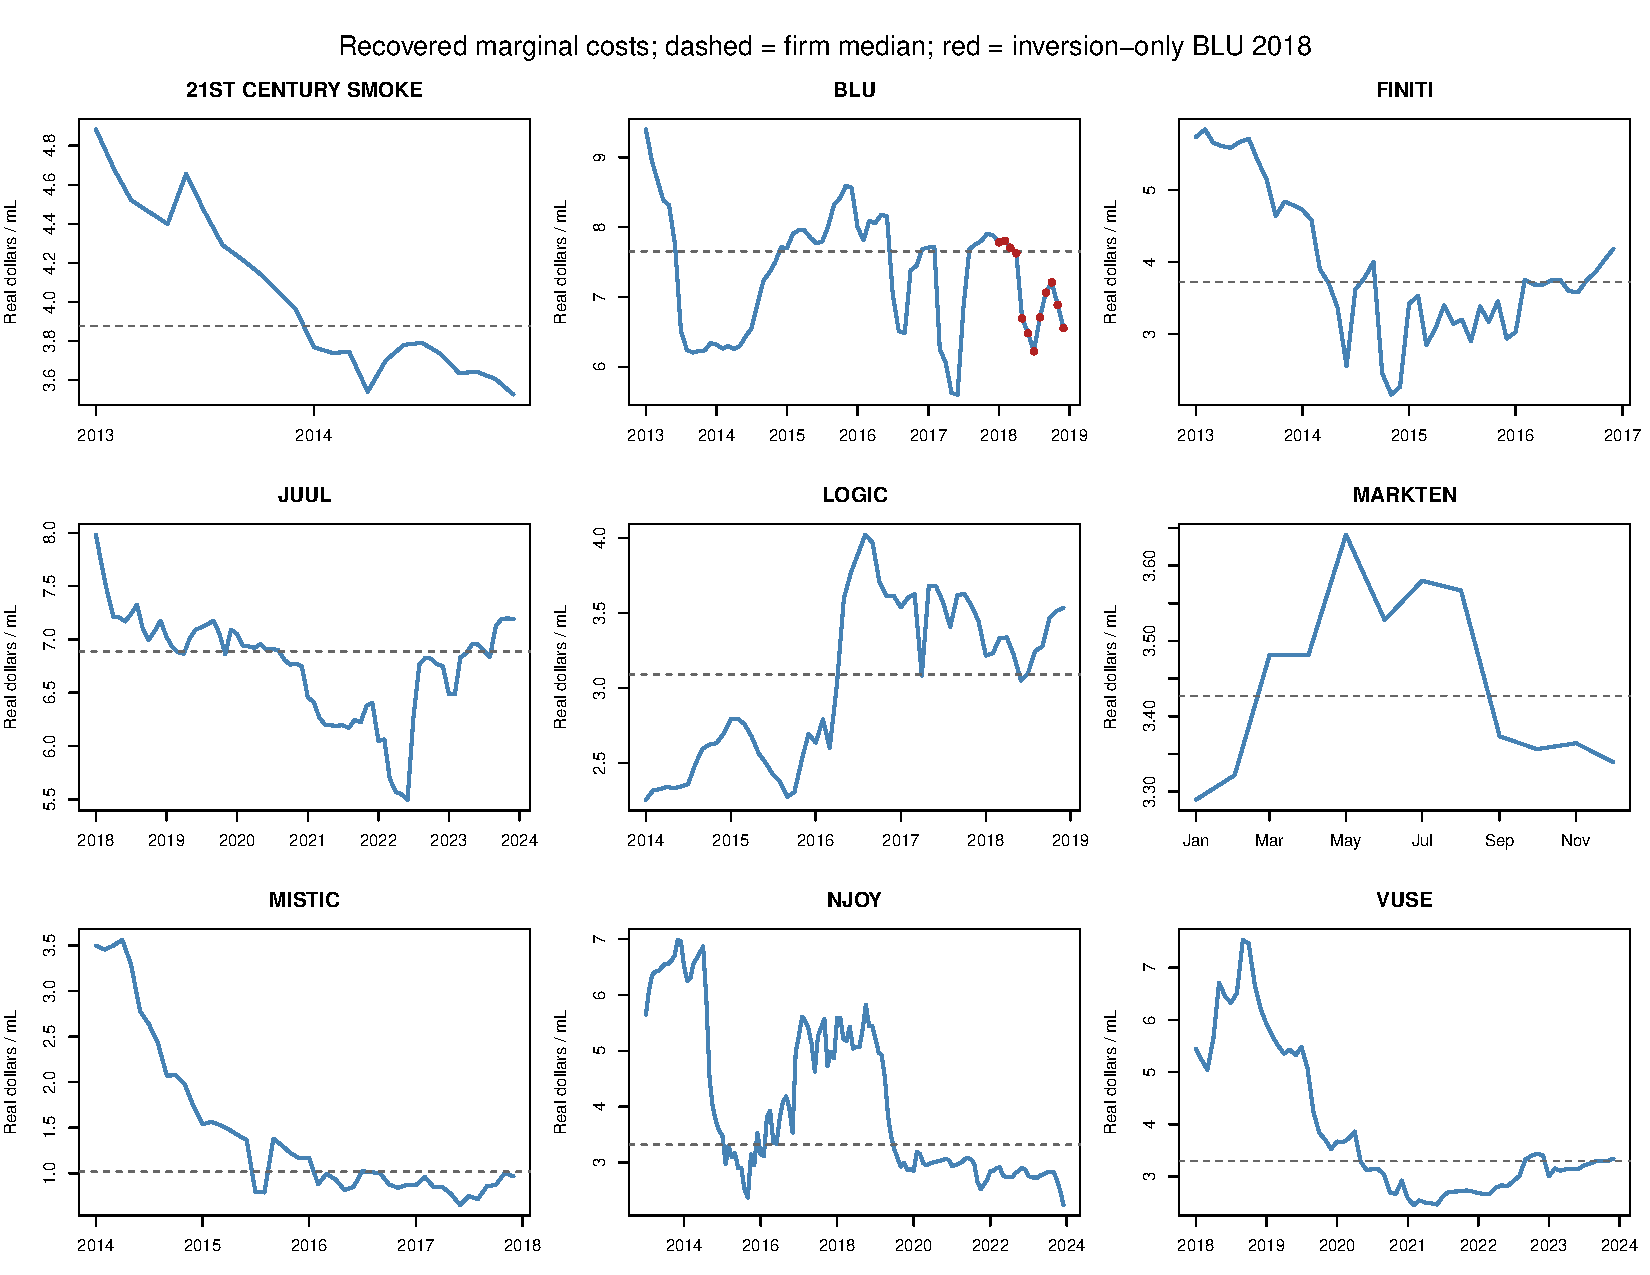
\includepdf[pages=-,landscape=true,fitpaper=true,pagecommand={}]{../../output/dynamic_entry_exit/marginal_cost_audit_2026-11-03/recovered_marginal_cost_audit.pdf}

\end{document}
